\documentclass{article}
\usepackage{fancyhdr} %For Header & footer Horizontal lines
\pagestyle{fancy} %For Header & footer Horizontal lines
\usepackage{lmodern}
\usepackage{pdfpages}
\usepackage{amsmath}
\usepackage[a4paper, left=0.5in, right=0.5in, top=0.5in, bottom=0.5in]{geometry}
% \usepackage[utf8]{inputenc}
\usepackage{graphicx}
\usepackage{times}
\usepackage{hyperref}
\usepackage{float}
\usepackage{xurl}
\usepackage{array} % For better column formatting

% Header and footer line thickness
\renewcommand{\headrulewidth}{0.4pt}
\renewcommand{\footrulewidth}{0.4pt}
\fancyhfoffset[L,R]{0pt} % Removes header and footer side offsets

\begin{document}

\begin{figure}
    
\includegraphics[width=0.1\textwidth]{images/UOJ_New_Logo_Transparent.png}
\end{figure}

\begin{figure}
    \centering
    
\includegraphics[width=0.2\textwidth]{images/Haircut_icon.png}
    \caption{Haircut application Icon}
\end{figure}
    \label{fig: App icon}
    \begin{table}[h] % Place the table "here" (h) on the page
        \centering
        \begingroup
    \fontsize{15}{20}\selectfont
    \begin{tabular}{|c |c|} \hline  % Define the number of columns and their alignment
        \textbf{\fontsize{18}{20}\selectfont Name(s)}& \textbf{\fontsize{18}{20}\selectfont ID(s)}\\ \hline         
       Marwan Almehmadi& 1741630
\\ \hline 
        Anas Aldhahri& 1845490\\ \hline 
        
 Waleed Aldhahri&2042395\\ \hline 
 Abdulrahman Maghrabi&2042791\\ \hline 
 Ali Abualwah&2140185\\ \hline 
 Sari Alblwi&2142407\\ \hline
    \end{tabular}
    \caption{Names and IDs}
    \label{tab:yourtablelabel}

    \vspace{1em}\begin{tabular}{|c |c|} \hline
    \textbf{Supervisor}&Dr. Sakher Ghanem\\ \hline
    \end{tabular}

    \vspace{3em}\begin{tabular}{|c|} \hline
        University of Jeddah \\
        College of Computer Science and Engineering \\
        Department of Computer Science\\
        Academic Session: Spring 2024 \\ \hline
    \end{tabular}
    \endgroup
\end{table}
\newpage
\section{Report Outline:}
\subsection{Chapter 1: General Presentation} 
\begin{itemize}
    \item \textbf{Introduction:} A general introduction of the proposed service.
    \item \textbf{General Context:} A description of the general context of the services.      
    \item \textbf{Problem Definition:} The problem the service offers to solve.
    \item \textbf{Aims:} General goals of the service.
    \item \textbf{Objectives:} List of measurable objectives which should be satisfied for the service to meet its aims.
    \item \textbf{Proposed Solution:} A brief description of the proposed solution the service offers.
    \item \textbf{Project Plan:} Approximate timetable of the project progress.
\end{itemize}
\subsection{Chapter 2: Related Works}
\begin{itemize}
    \item \textbf{Introduction:} An introduction to the domain of the service.
    \item \textbf{Background:} ho is the service is targeting.
    \item \textbf{Literature Review:} A literature review describing the features of the system, from multiple sources.
    \item \textbf{Existing Systems:} Services that share the same domain and their advantages \& disadvantages.
    \item \textbf{Comparison:} Comparison between the services at hand \& other services share the same domain.
    \item \textbf{Conclusion:} Conclusion of the report.
\end{itemize}
\subsection{Chapter 3: General Analysis}
\begin{itemize}
    \item \textbf{Introduction:} A general introduction of the analysis. Analysis serves as a fundamental tool for exploring patterns, trends, and relationships.
    \item \textbf{Requirements Gathering:} A description of how the requirements have been gathered.
    \item \textbf{Functional Requirements:} The Requirements that the system needs to function.
    \item \textbf{Non-functional Requirements:} The Requirements that are expected to be in the system.
    \item \textbf{Use Case Diagram:} A display of a use case diagram.
    \item \textbf{Dynamic Diagram:} A display of a dynamic diagram, in this case an activity diagram.
    \item \textbf{Conclusion:} Conclusion of the chapter.
\end{itemize}
      \subsection{Chapter 4: Detailed Desgin}
\begin{itemize}
    \item \textbf{Introduction:} An introduction to the detailed design chapter
    \item \textbf{Static Aspect Design:} A display of a class diagram for designing functional requirements and reflecting non-functional requirements.
    \item \textbf{Architectural Aspect Design:} A presentation of the different hardware components of the proposed solution.
    \item \textbf{Dynamic Aspect Design:} A detailed diagram to reflect the internal dynamic of the proposed functional requirements.
    \item \textbf{User Interface Design:} A display of the user interface design and screens.
    \item \textbf{Conclusion:} Conclusion of the report.
\end{itemize}\pagebreak
\section{Chatper 1: }
      \subsection{Introduction:}
      In the age of technology \& fast pace of living, it’s becoming increasingly challenging day after day for manual professions, leaving pursuers of such jobs a challenging journey amidst shifting economics \& environmental factors, due to the constant utilization of tasks, pursuers of such jobs are left with no choice except to take the surfboard of modern technology and ride the waves of progression, even though some of these jobs are still in demand, However, due to the random unaccounted-for approaches to the domain \& unregulated processes involved in these kinds of jobs, which results in missed opportunities, wasted time, unsatisfied customers due poor communication, etc. this proposal discusses \& offers a services solutions to one of this domain issues which are barbershops.
      \subsection{General Context}
      \textbf{Haircut:} A service that improves the profession of barbers by taking advantage of technology to minimize wasted efforts and time \& to create a better experience for both customers \& barbers. The service provides appointments, a rating system, age range, a communication system, a payment system and a sign-up option to provide the barbers and customers with a better experience and to achieve the overall satisfaction of the services provided.
      \subsection{Problem Definition: }
      Minimizing wasted time for customers in barbershops domain and increasing customer’s satisfaction while improving \& serving the profession as legitimate career.
      \subsection{Aims: }
      \begin{itemize}
        \item Minimizing the customers' dissatisfaction.
        \item Improving the barber profession by taking advantage of technology \& ease the process to the customers.
        \item Giving more chance for barbers to offer their services responding for customers' orders that aren’t necessarily tied to the barbershop place.
        \item The user can order a barber appointment into his home for people and elders who have movement issues or kids, also people who lack transportation means .
        \item Improving the profession by minimizing the following:
        \begin{itemize}
            \item Health risks for both customers and barbers.
            \item Barbers: 
            \begin{itemize}
                \item Avoiding long stands by setting a timer for each session.
            \end{itemize}
            \item Customers:
            \begin{itemize}
                \item The customer guarantees the cleanliness of tools in each session.
            \end{itemize}
            \item Waiting Time
            \begin{itemize}
                \item Customer can check the occupancy level of a barbershop.
            \end{itemize}
        \end{itemize}
      \end{itemize}
      \subsection{Objectives:}
      \begin{itemize}
        \item A variety of services options offered to customers from the barbershop.
        \item Ability for customer the price for services.
        \item Ability for Barbers to rate customers.
        \item Statistics of time spent daily \& number of customers served.
        \item Providing the ability of reserving an appointment in a barbershop instead of manually waiting in line.
        \item A professional certificate for a barber.
        \item Signing an agreement to comply with the profession's regulations.
        \item User agreement of sharing data such as phone number and email address as an opportunity to enhance the service for a better experience.
        \item Shaving tools sold from suppliers to serve both customers and barbers.
        \item  Recommendations for customers to enhance their experience.  
      \end{itemize}
      \subsection{Proposed Solution:}
      This service will serve as a business marketing tool for barbershops and time-saving tool for customers, by providing multiple tools and options to help both customers and barbers to achieve their desired satisfaction. It serves the Barber, the customers, the barber shop, and the suppliers.
      \begin{itemize}
        \item \textbf{For Customers:} The app helps the customers by providing options for both indoor and outdoor barber services and making appointments for the respective services.
        \item \textbf{For Barbers:} The app helps the barbers ensure that they can find multiple opportunities to make their services available, both inside and outside the barber shop.
        \item \textbf{For Barber shops:} The app helps the barber shop increase their customer count, less waiting time for customers, more revenue for the barber shop, and finally overall customer satisfaction.
        \item \textbf{For suppliers:} The app helps the suppliers advertise their products for both customers and barbers, to achieve the desired profit/revenue from selling their products.           
      \end{itemize}

      \subsection{Project Plan:}
      \begin{figure}[H]
          \centering
          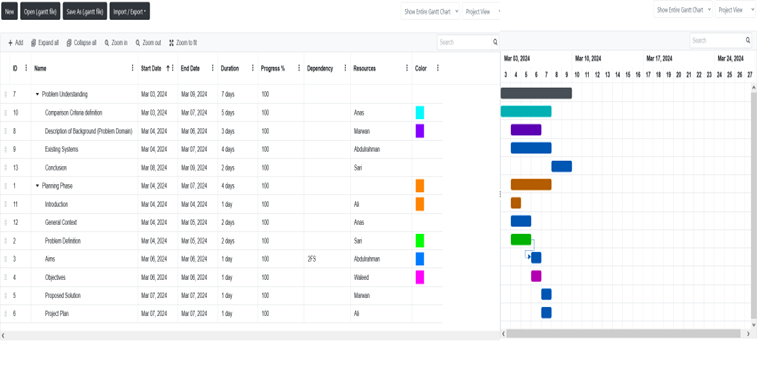
\includegraphics[width=1\linewidth]{images/Project_plan.png}
          \caption{Project Plan }
      \end{figure}
      \newpage
      \section{Chapter 2: Related Works}
      \subsection{Introduction:}This chapter will cover other services that share the same domain, their pros and cons and the difference between them.
      \subsection{Background:}We are going to explain the existing systems, the pros, and cons of each existing system, and how our project will avoid the cons and improve the pros if applicable. Starting with the \textbf{\textit{pros}} of each existing system. The first pro/advantage is the \textbf{\textit{User-Friendly Interface}}, it is provided by \textit{Acuity Scheduling, Mindbody, Vegaro, WellnessLiving, Setmore, StyleSeat, }and \textit{Schedulicity. }The second pro/advantage is \textbf{\textit{Convenient Appointment Booking}}\textit{, }it is provided by \textit{Acuity Scheduling, Vegaro, WellnessLiving, TheCut app, StyleBeat and Schedulicity. }The third pro/advantage is \textbf{\textit{Automated Reminders, }}it is provided by \textit{Acuity Scheduling, Setmore, }and \textit{Square Appointments. }The fourth pro/advantage is the\textbf{\textit{ Payment System}}, it is provided by\textit{ Mindbody and Zenoti. }The fifth pro/advantage is the\textbf{\textit{ Rating /Review System, }}provided by \textit{StyleSeat. }Now with the \textbf{\textit{cons}} of the existing systems. The first con/disadvantage is the \textbf{\textit{Pricing}}, the existing systems that have pricing issues are \textit{Acuity Scheduling, Zenoti }and \textit{StyleSeat. }The second con/disadvantage is the \textbf{\textit{Learning Curve, }}the existing systems that have learning curve issues are \textit{Acuity Scheduling} and \textit{Zenoti}. The third con/disadvantage is the Browser Sensitivity, the existing systems that have browser sensitivity issues are WellnessLiving and Schedulicity. The fourth con/disadvantage is the \textbf{\textit{Credit Card Swiping Feature}}, the existing systems that lack the credit card swiping feature are \textit{WellnessLiving }and\textit{ Schedulicity}.
      Our project aims to minimize or avoid the provided cons, and work to improve the provided pros, there is a feature we would like to add, and it is the \textbf{\textit{Communication System}} which allows both customers and barbers to communicate with each other through messages or a phone call. We also found that there aren't any existing systems in the Middle east, so our project might be the first existing system in the Middle east.   
      \subsection{Literature Review:}In this section, we are going to review the features of our project and a description of each feature and some related articles and researches, starting with the home service feature, user-friendly interface, convenient appointment booking, automated reminders, payment system, and finally rating/review system.
      \begin{itemize}
        \item \textbf{1- }\textbf{Home Service: }for this feature, we have found an academic article that describes their discovery on a home service consumption, InHoServ provides a comprehensive understanding of the main actors involved in-home service consumption and delineates their changing role. \textbf{(Tsiotsou \& Boukis, 2022)}
        \item \textbf{2- }\textbf{User-Friendly Interface: }for this feature, we have found a research article about HCI that describes the patterns needed for a user friendly interface, that includes the \textbf{usability}: A usable product seeks to achieve three main outcomes: (1) the product is easy for users to become familiar with and competent in using it during the first contact, (2) the product is easy for users to achieve their objective through using it, and (3) the product is easy for users to recall the user interface and how to use it on later visits. \textbf{The User Experience}: Basically, an important concept in UX is the process by which users form experiences since they first encounter the product and as the product is used throughout a period. \textbf{The User Diversity}: It is the process of creating products that can be accessed by as many people as possible, for example, people with disablilities. (\textbf{Hindawi,2017).}
        \item \textbf{3- }\textbf{Convenient Appointment Booking}: for this feature we have found a research article about an appointment booking for hospitals, and some advantages of having a hospital management system for appointments: (1) Simple patient information recovery: HMS makes it conceivable to get to all the information identified with a patient, data like patient history, current sickness, specialists included, tests reports taken, charging data and a lot more can be made obvious to the client, (2) Improve Visibility and Transparency: Medical clinic Management System (HMS) improves the deceivability and straightforwardness in the total Administration measure and in all records. (3) Simplicity to Access System Facilities: Medical clinic Management System makes it simple to gain Admittance to the Administration framework Offices for the approved clients and protect it from unapproved clients. \textbf{(Sarita Priyadarshini Nayak \& Bharat Bhushan, 2021)}
        \item \textbf{4- }\textbf{Automated Reminders: }for this feature we have found an article that describes automated reminders targeting patients in a hospital, Alerts have been used to notify a physician of a contraindicating condition like an allergy, interaction with another medication or supplement (immediate alert), or to prompt a clinician to respond to an abnormal lab value (event-driven alert).[8] Reminders have been used to notify clinicians and patients supposedly through SMS about appointments like preventive screenings or vaccinations. An electronic literature search was conducted in the PubMed database to identify studies on electronic interventions in the form of alerts and reminders targeted specifically for patients\textbf{.(} \href{https://pubmed.ncbi.nlm.nih.gov/?term=Perri-Moore\%20S\%5BAuthor\%5D}{\textbf{Seneca Perri-Moore}}, PhD, RN,\textbf{\textsuperscript{1,*}} \href{https://pubmed.ncbi.nlm.nih.gov/?term=Kapsandoy\%20S\%5BAuthor\%5D}{\textbf{Seraphine Kapsandoy}}, PhD, RN,\textbf{\textsuperscript{2}} \href{https://pubmed.ncbi.nlm.nih.gov/?term=Doyon\%20K\%5BAuthor\%5D}{\textbf{Katherine Doyon}}, MS,\textbf{\textsuperscript{3}} \href{https://pubmed.ncbi.nlm.nih.gov/?term=Hill\%20B\%5BAuthor\%5D}{\textbf{Brent Hill}}, PhD, RN,\textbf{\textsuperscript{1}} \href{https://pubmed.ncbi.nlm.nih.gov/?term=Archer\%20M\%5BAuthor\%5D}{\textbf{Melissa Archer}}, PharmD,\textbf{\textsuperscript{4}} \href{https://pubmed.ncbi.nlm.nih.gov/?term=Shane-McWhorter\%20L\%5BAuthor\%5D}{\textbf{Laura Shane-McWhorter}}, PharmD,\textbf{\textsuperscript{4}} \href{https://pubmed.ncbi.nlm.nih.gov/?term=Bray\%20BE\%5BAuthor\%5D}{\textbf{Bruce E. Bray}}, MD, PhD,\textbf{\textsuperscript{1}}\textbf{ and }\href{https://pubmed.ncbi.nlm.nih.gov/?term=Zeng-Treitler\%20Q\%5BAuthor\%5D}{\textbf{Qing Zeng-Treitler}}, PhD\textbf{\textsuperscript{1}}, 2016)\pagebreak
        \item \textbf{5- }\textbf{Payment System:} for this feature, we have found a review on an E-payment system in E-commerce, An electronic payment system comes to replace a cash payment system [17] , E-Payment is a system that provides tools for payment of services or goods carried on the internet [10]. It provides the ease of transaction processing in e-commerce between consumers and sellers [16]. Using the E-payment System has many benefits for payers, payees, E-commerce, banks, organizations, and governments. These benefits can lead to widespread electronic payment systems in the world [32]. \textbf{(}\href{https://www.researchgate.net/profile/Ferry-Wibowo?_tp=eyJjb250ZXh0Ijp7ImZpcnN0UGFnZSI6InB1YmxpY2F0aW9uIiwicGFnZSI6InB1YmxpY2F0aW9uIn19}{\textbf{Ferry Wahyu Wibowo}}\textbf{,2018)}
        \item \textbf{6- }\textbf{Rating/Review System}: for this feature, we have found a research article that provides a similar topic to ours, app stores commonly employ simple rating mechanisms, in at least five of the most popular app-stores, which are Apple's app store ,Google Play, Windows Phone store , Amazon Appstore, and Blackberry App World (now defunct), the store rating is represented as a number of "stars" from 1 to 5, aggregated from individual user ratings. In Google play, the store-rating of an app is the cumulative average of all individual user ratings given to the app over all versions. \textbf{(}\href{https://www.researchgate.net/profile/Bram-Adams?_tp=eyJjb250ZXh0Ijp7ImZpcnN0UGFnZSI6InB1YmxpY2F0aW9uIiwicGFnZSI6InB1YmxpY2F0aW9uIn19}{\textbf{Bram Adams}}\textbf{, Israel Mojica Ruiz, }\href{https://www.researchgate.net/scientific-contributions/Meiyappan-Nagappan-65898809?_tp=eyJjb250ZXh0Ijp7ImZpcnN0UGFnZSI6InB1YmxpY2F0aW9uIiwicGFnZSI6InB1YmxpY2F0aW9uIn19}{\textbf{Meiyappan Nagappan}}\textbf{, }\href{https://www.researchgate.net/scientific-contributions/Thorsten-Berger-2005390073?_tp=eyJjb250ZXh0Ijp7ImZpcnN0UGFnZSI6InB1YmxpY2F0aW9uIiwicGFnZSI6InB1YmxpY2F0aW9uIn19}{\textbf{Thorsten Berger}}\textbf{,} \textbf{Ahmed E. Hassan, 2017)}  
      \end{itemize}\pagebreak
      \subsection{Existing Systems:}
      \subsubsection{Acuity Scheduling:}
      Acuity Scheduling is a powerful online appointment scheduling tool designed to streamline and simplify the booking process for businesses and service providers. With the following features Appointment Scheduling:
      \begin{itemize}
      \item \textbf{Client-Friendly}: Acuity makes it easy for clients to book appointments. Once the client set up his/her account, clients can schedule appointments seamlessly.
      \item \textbf{Customizable Appointment Types}: the client can create different appointment types (e.g., initial consult, follow-up) with various settings:
        \begin{itemize}
            \item Name the appointment.
            \item Add a description.
            \item Set a duration.
            \item Specify a price.
            \item Organize appointment types into categories.
            \item Upload a photo.
            \item Add intake forms for clients.
            \item Availability Control: Customize when clients can book by setting limits:
            \item Choose specific days and times.
            \item Set advance booking requirements.
            \item Prevent last-minute cancellations or rescheduling.
            \item Limit daily or weekly appointments.
            \item Block off vacation days or personal time.
            \item Automatic Time Zone Conversion: Acuity detects and converts time zones, eliminating confusion when scheduling across different regions.
            \item Add-Ons \& Upsells.  
        \end{itemize}
      \end{itemize}
      \textbf{Reference}: \href{https://acuityscheduling.com/\#gref}{https://acuityscheduling.com/\#gref} 
      \subsubsection{DaySmart Salon.}
      DaySmart Salon is a robust software solution designed to enhance the management and efficiency of salons, spas, barbershops, nail salons, and other industry-related businesses. The app features are:
      \begin{itemize}
        \item Appointment Scheduling and Business Management:
        \item Versatile Booking App: Formerly known as Salon Iris, DaySmart Salon offers powerful scheduling and business management capabilities.
        \item For Various Business Sizes: Whether the client run a small hair salon or a large spa, this app suit the client’s needs.
        \item ­­­Mobile Access: the client can manage his/her salon on-the-go using your iPad, iPhone, Android, or web browser.
        \item 24/7 Appointment Management: View, add, or edit appointments from anywhere, anytime.
        \item Remote Business Control: Access over 25 essential features, including business reports, appointment books, payroll totals, marketing, and text messaging.  
      \end{itemize}
      Key Features:
    \begin{itemize}
        \item Efficient Day Management: Free up time by streamlining daily processes.
        \item Client-Centric Approach: Keep clients top-of-mind while handling administrative tasks.
        \item Cloud-Based Solution: Access everything from the front desk or your mobile device.
        \item Designed for Salons and Spas: DaySmart Salon caters exclusively to the salon and spa industry.
    \end{itemize}
      Benefits:
      \begin{itemize}
        \item Time Savings: Automate communication, appointment scheduling, and reporting.
        \item Engage Staff: Modern technology keeps your team connected.
        \item Business Growth: Efficient management allows you to focus on expanding your business.  
      \end{itemize}      
      \textbf{Reference}: \href{https://www.daysmart.com/salon/}{https://www.daysmart.com/salon/}
      \subsubsection{Mindbody:}
      The Mindbody app is a powerful tool that connects consumers with fitness, beauty, and integrative health businesses. Whether you’re a business owner or a wellness enthusiast, here’s an in-depth look at what the Mindbody app offers:
      Overview: The Mindbody app is a free mobile app available for both iOS and Android devices. Its primary purpose is to help users find and explore various wellness services, including fitness classes, beauty treatments, and integrative health practices.
      As a business owner, you can use the app to manage bookings, attract new clients, and enhance your brand visibility.
      Features and Benefits:
      Business Listings: The app showcases listings of fitness studios, salons, spas, and other wellness providers. Users can search by service type, zip code, or business name.
      Booking Services: Existing clients can easily book appointments through the app, streamlining the scheduling process.
      Discover New Businesses: New customers can discover your business through the app, making it a valuable platform for attracting fresh clientele.
      Keyword Optimization: Businesses can optimize their listings with relevant keywords to improve visibility during searches.
      Flexible Pricing: The app features dynamically priced drop-ins, making it easier for users to find available spots and classes.
      Categories and Subcategories: Properly categorizing your services helps users quickly find what they’re looking for.
      Surge Pricing: Businesses can use surge pricing to maximize revenue during high-demand periods.
      For Business Owners:
      Maximize Earning Potential: Craft an irresistible listing that showcases your brand and services.
      Keyword Optimization: Use descriptive keywords to ensure your business appears in relevant searches.
      Flexible Pricing: Set up dynamically priced drop-ins to enhance visibility.
      Categories and Subcategories: Select the right categories for your classes and appointments.
      Surge Pricing: Optimize revenue during peak times.
      For Users:
      Search and Explore: Users can find nearby fitness classes, beauty treatments, and wellness services.
      Booking Convenience: Easily book appointments and manage their wellness routines.
      Personalized Recommendations: The app suggests relevant services based on user preferences.
      Community Connection: Connect with like-minded individuals and explore new wellness experiences.
      In summary, the Mindbody app bridges the gap between wellness businesses and consumers, making it a valuable resource for both parties. Whether you’re a business owner or someone seeking wellness services, the app offers convenience, visibility, and a vibrant community of enthusiasts.\newline
      \textbf{Reference}: \href{https://www.mindbodyonline.com/en-gb/business/lp/mindbody?landing=y&utm_source=google&utm_medium=ppc&utm_campaign=20430748488&ad_group=160722387588&utm_term=kwd-329860702&utm_device=c&referralSource=paid+search&matchtype=e&cid=685008699808&networkType=search&adgroupid=160722387588&creative=685008699808&network=g&adGroup=160722387588&_bk=mindbody&_bm=e&gad_source=1&gclid=Cj0KCQiArrCvBhCNARIsAOkAGcXkhoxZN2kd43kY-JN37kZmb38xqd5jLQhS4T8uUtLw5eR_OVGaqy4aAlL3EALw_wcB}{MindBodyOnline}

      \subsubsection{Vagaro.}
      Vagaro is a comprehensive software solution designed for salons, spas, fitness centers, and other wellness businesses.
      It offers both mobile apps for business employees and a customer-facing app for clients.
      Available on iOS and Android, Vagaro streamlines appointment booking, management, and communication.
      Features for Business Owners:
      Appointment Booking: Business owners can manage appointments seamlessly.
      Client Management: Keep track of client details, preferences, and history.
      Marketing Tools: Promote services through email campaigns, loyalty programs, and social media integration.
      Point of Sale (POS): Process payments, track inventory, and manage sales.
      Reports and Analytics: Access insights on revenue, client retention, and performance.
      Staff Management: Schedule employees, track commissions, and monitor productivity.
      Customizable Listings: Create an attractive business profile with photos, services, and pricing.
      Online Booking: Clients can book appointments directly through the app.
      Features for Clients:
      Discover Services: Users can explore nearby salons, spas, and fitness centers.
      Book Appointments: Easily schedule appointments based on availability.
      View Ratings and Reviews: Check ratings and read reviews from other clients.
      Receive Reminders: Get notifications for upcoming appointments.
      Secure Payments: Pay for services within the app.
      Loyalty Programs: Participate in loyalty programs and earn rewards.
      Community Engagement: Connect with other users and share experiences.
      Strengths:
      User-Friendly: Intuitive interface for both clients and business owners.
      Comprehensive: Covers all aspects of salon and wellness management.
      Mobile Access: Manage business operations on the go.
      Marketing Tools: Boost client engagement and retention.
      Client-Centric: Enhances the client experience.
      Limitations:
      Pricing: Some users find the pricing structure complex.
      Learning Curve: New users may need time to explore all features.
      Customization: Limited customization options for certain features.
      Pricing:
      Vagaro offers different pricing tiers based on business needs.
      Visit the official Vagaro website for detailed pricing information1.
      In summary, Vagaro empowers businesses to efficiently manage appointments, engage clients, and enhance their overall operations. Whether you’re a salon owner or a wellness enthusiast.\newline
      \textbf{Reference}: \href{https://www.vagaro.com/pro/about-us}{https://www.vagaro.com/pro/about-us}
      \pagebreak
      \subsubsection{WellnessLiving.}
      Overview:
      WellnessLiving offers the Achieve Client App, a powerful mobile app designed for both business owners and clients in the wellness industry.
      Available on iOS and Android, this app streamlines appointment booking, engagement, and business management.
      Features for Business Owners:
      Custom Branded App: Create your own branded app to enhance your business’s visibility and streamline online bookings.
      Client Management: Keep track of client details, preferences, and history.
      Marketing Tools: Promote services through email campaigns, loyalty programs, and social media integration.
      Point of Sale (POS): Process payments, track inventory, and manage sales.
      Reports and Analytics: Access insights on revenue, retention rates, and performance.
      Staff Management: Schedule employees and monitor productivity.
      Virtual Training Solutions: Take your services online with virtual sessions and on-demand classes.
      Features for Clients:
      Booking Services: Clients can easily find and book appointments at your studio.
      Reward Points: Collect points and redeem them for prizes.
      Account Management: Update account details and make purchases directly from the app.
      Notifications: Receive reminders and change notifications for upcoming classes and appointments.
      Benefits:
      Brand Consistency: Customize your app with fonts, colors, and images to maintain brand identity.
      Real-Time Booking: Clients can book classes, appointments, and events instantly.
      Sales and Payments: Access your online store, purchase memberships, and store credit cards.
      Client Engagement: Use push notifications for promotions, loyalty discounts, and announcements.
      Rewards Program: Incentivize clients to refer friends and share experiences.
      Reviews and Reputation:
      Encourage happy clients to review your business within the app to attract new leads.
      In summary, the WellnessLiving Achieve Client App bridges the gap between wellness businesses and clients, offering convenience, engagement, and brand recognition. Whether you’re a business owner or a wellness enthusiast, this app provides a holistic solution!\newline
      \textbf{Reference}: \href{https://www.wellnessliving.com/}{https://www.wellnessliving.com/}

      \subsubsection{Zenoti.}
      The Zenoti app is your go-to all-in-one comprehensive salon and spa management system.
      Designed for both business owners and clients, it streamlines various aspects of wellness businesses.
      Available on iOS and Android, Zenoti empowers businesses to thrive and clients to enjoy seamless experiences.
      Features for Business Owners:
      Custom Branded App: Create your own branded app to enhance visibility and streamline online bookings.
      Client Management: Keep track of client details, preferences, and history.
      Marketing Tools: Promote services through email campaigns, loyalty programs, and social media integration.
      Point of Sale (POS): Process payments, track inventory, and manage sales.
      Reports and Analytics: Access insights on revenue, retention rates, and performance.
      Staff Management: Schedule employees, track commissions, and monitor productivity.
      Virtual Training Solutions: Take services online with virtual sessions and on-demand classes.
      Features for Clients:
      Booking Services: Easily find and book appointments at your preferred salon or spa.
      Reward Points: Collect points and redeem them for prizes.
      Account Management: Update details and make purchases directly from the app.
      Notifications: Receive reminders and change notifications for upcoming appointments.
      Benefits:
      Brand Consistency: Customize the app with your brand’s fonts, colors, and images.
      Real-Time Booking: Clients can book classes, appointments, and events instantly.
      Sales and Payments: Access your online store, purchase memberships, and store credit cards.
      Client Engagement: Use push notifications for promotions, loyalty discounts, and announcements.
      Rewards Program: Incentivize clients to refer friends and share experiences.
      Reviews and Reputation:
      Encourage happy clients to review your business within the app to attract new leads.
      In summary, Zenoti bridges the gap between wellness businesses and clients, offering convenience, engagement, and brand recognition.\newline
      \textbf{Reference}: \href{https://www.zenoti.com/}{https://www.zenoti.com/}

      \subsubsection{TheCut App}
      TheCut is a powerful barber booking app that simplifies the process of finding talented barbers and scheduling haircuts. Whether you’re a client looking for a fresh trim or a barber managing appointments, here’s an in-depth look at what TheCut offers: For Clients:
      Discover Barbers: TheCut connects you with over 15,000 barbers across the US.
      Easy Booking: Schedule your next haircut effortlessly.
      Flexible Occasions: Book for same-day cuts, house calls, weddings, or while traveling.
      Notifications: Receive reminders and updates about your appointments.
      For Business Owners (Barbers):
      Digital Booth Setup: Create your digital presence in just 5 minutes.
      Booking Management: Easily manage your schedule.
      Brand Building: Strengthen your brand identity.
      Digital Payment: Process payments seamlessly.
      Push Notifications: Keep clients informed.
      24/7 Calendar Management: Stay organized.
      Referrals and Rewards: Encourage client referrals.
      Client Reviews: Showcase positive feedback.
      Analytics Dashboard: Access performance insights.
      In summary, TheCut modernizes men’s grooming by connecting clients with skilled barbers. Whether the user is seeking a fresh look or a barber managing appointments, TheCut simplifies the process and enhances the industry experience!\newline
      \textbf{Reference}: \href{https://www.thecut.co/}{https://www.thecut.co/}
      \subsubsection{Setmore}
      Setmore is a free online customer appointment scheduling tool that simplifies the process of booking appointments with your clients. Whether you’re a hair stylist, a personal trainer, or a wellness practitioner, Setmore provides a comprehensive solution for managing your appointments and enhancing your business. Let’s dive into the details:
      Calendar:
      The calendar is the heart of Setmore. Here’s what it offers:
      Booking Appointments: Easily schedule appointments by clicking on available time slots.
      Staff Calendars: Each staff member has their own calendar, allowing you to manage multiple schedules.
      Availability: White space represents your working hours, while grey space indicates non-working hours.
      Current Day Indicator: A floating red line shows the current day and time.
      Customer List:
      Your customer list acts as a digital rolodex:
      Client Details: Includes customer names, contact information, and appointment history.
      Custom Fields: Add custom form fields to capture additional data.
      Behavioral Insights: View lifetime value, average purchases, and services purchased over time.
      Booking Page:
      Every Setmore account comes with a free Booking Page:
      Public-Facing Web Page: Lists your services, staff, availability, and contact info.
      Customization: Upload your business logo and add a Google Maps pin.
      Self-Booking: Share or embed the Booking Page on your website, allowing clients to book appointments without calling you.       
      Notifications:
      Setmore sends notifications to keep you and your clients informed about upcoming appointments and changes.
      Staff Profiles:
      Manage your team by creating individual staff profiles:
      Services Offered: Specify the services each staff member provides.
      Availability: Set working hours and breaks.
      Booking Preferences: Customize booking rules for each staff member.
      Benefits:
      Time Organization: Setmore helps you organize your time effectively.
      Client Management: Keep track of client interactions and preferences.
      Brand Visibility: Customize your Booking Page to reflect your brand.
      Self-Booking: Clients can book appointments without hassle.
      Insights: Understand your best customers and their behaviors.
      a fully booked Setmore calendar reflects the health of the user’s business. Whether the user is a solo practitioner or a manager of a team, Setmore streamlines appointment management and enhances client experiences!\newline
      \textbf{Reference}: \href{https://www.setmore.com/}{https://www.setmore.com/}
      
      \subsubsection{StyleSeat}
      StyleSeat is a beauty and grooming marketplace that caters to both clients and beauty professionals. Let’s explore its features and benefits:
      For Clients:
      Discover and Book Appointments: Clients can easily search for and book appointments with beauty and barber professionals.
      Flexible Booking: Whether it’s a same-day blowout, a haircut next month, or a manicure tomorrow, StyleSeat allows clients to find available slots.
      Notifications: Clients receive helpful appointment reminders.
      Browse Photos and Reviews: Explore hairstyles, colors, and reviews to make informed choices.
      Recurring Appointments: Set up recurring appointments with your favorite barber or stylist.
      For Beauty Professionals (Barbers, Stylists, etc.):
      Digital Booth Setup: Create your digital presence quickly.
      Booking Management: Efficiently manage your schedule.
      Brand Building: Customize your profile to reflect your brand.
      Payments and Pricing: Process payments seamlessly.
      Notifications: Keep clients informed about changes.
      Calendar Management: Organize your time effectively.
      Client Reviews: Showcase positive feedback.
      Analytics Dashboard: Access performance insights.
      Why StyleSeat Is Essential for Independent Professionals:
      Time Savings: StyleSeat handles administrative tasks, allowing you to focus on services.
      Online Service Menu: Clients can explore your services and pricing without inquiries.
      Self-Booking: Clients schedule appointments directly, reducing phone calls and texts.
      Business Insights: Understand your best clients and their behaviors.
      In summary, StyleSeat empowers both clients and professionals by streamlining appointment management, enhancing brand visibility, and fostering a vibrant beauty community!\newline
      \textbf{Reference}: \href{https://www.styleseat.com/m/}{https://www.styleseat.com/m/}
      
      \subsubsection{Square Appointments}
      Square Appointments is a comprehensive scheduling and booking app designed to streamline appointment management for businesses. Here’s an overview of its features and functionalities:
      Scheduling and Availability Management:
      Manage Availability: You can control your availability directly from the app. Set your working hours, breaks, and days off.
      Online Booking: Enable customers to book appointments or classes online through a custom booking website.
      Waitlists: Fill gaps in your schedule due to last-minute cancellations or reschedules with waitlists.
      Point of Sale (POS):
      Flexible Checkout Options: Check out at the counter, keep a card on file, or send an invoice.
      Card Payments: Integrated payment processing for seamless transactions.
      Client Profiles and Team Management:
      Client Profiles: Prioritize your customers by maintaining detailed profiles.
      Team Management: Organize your staff and assign responsibilities efficiently.
      Business Operations:
      Product Sales: Sell products both online and in-store. Sync your inventory and set up shipping.
      Customizable Pricing: Custom pricing and discounts are available for qualifying businesses.
      Industry-Specific Features:
      Square Appointments caters to various business types:
      Barbershops: For haircuts and life advice.
      Spas and Nail Salons: For self-care enthusiasts.
      Fitness Centers: For those who keep pushing.
      Health and Wellness Professionals: Specializing in health and healing.
      Professional Services: For expertise beyond internet learning.
      Home Repair and Cleaning Services: Saving homes from DIY disasters.
      Tutoring and Music Lessons: Believers in practice making perfect.
      Hair and Beauty Salons: Where magic happens with hair care.
      Pricing:
      Free Plan: Basics for running your business, including unlimited staff accounts, custom booking website, integrated payments, and automated reminders.
      Transaction Fees: 2.6\% + 10¢ per in-person transaction.
      Square Appointments simplifies the user’s administrative tasks, allowing the user to focus on what he/she love most about the business!\newline
      \textbf{Reference}: \href{https://squareup.com/us/en/appointments}{https://squareup.com/us/en/appointments}
      
      \subsubsection{Schedulicity}
      Schedulicity is an all-in-one scheduling software designed for busy service providers and small businesses. Let’s dive into the details:
      Appointment Booking and Management: Online Booking: Clients can seamlessly book appointments through the Schedulicity app.
      Master Calendar: View daily and weekly schedules, manage recurring, one-time, and last-minute bookings.
      Individual Calendars: Overview of up to 7 providers’ schedules at once.
      Client Check-Ins: Ideal for classes and workshops.
      Mobile Calendar Integration: Digital Calendar: Never miss an appointment with a fully synced calendar.
      Service Customization: List your services, customize policies, and track bookings.
      Waitlist Alerts: Fill gaps due to cancellations.
      Payment Processing: Convenient Transactions: Built-in payment processing for seamless transactions.
      Upsell Packages: Offer package deals during checkout.
      Contactless Payment: Experience pay-by-text and tipping options.
      Client Profiles: Comprehensive Client Information: Appointment history. Client notes. Pronoun preferences. Birthday. Payment details. Contact information. Industry-Specific Features:
      Schedulicity caters to various industries, including:
      Hair Salons: From Instagram-famous to local favorites.
      Nail Artists: Trendy and creative.
      Fitness Centers: Crossfit gyms and yoga studios.
      Wellness Professionals: Holistic health and healing.
      Professional Services: Expertise beyond online learning.
      Home Repair and Cleaning Services: Rescue from DIY disasters.
      Tutoring and Music Lessons: Perfecting skills.
      Beauty Salons: Where magic happens with hair care. Pricing: Free Plan: Includes unlimited staff accounts, custom booking website, integrated payments, and automated reminders.
      Transaction Fees: 2.6\% + 10¢ per in-person transaction.
      In summary, Schedulicity is an efficient appointment management system.\newline
      \textbf{Reference}: \href{https://www.schedulicity.com/}{https://www.schedulicity.com/}
      
      \subsection{Comparison}
      % Include specific pages (1 and 2) on a single page
      % 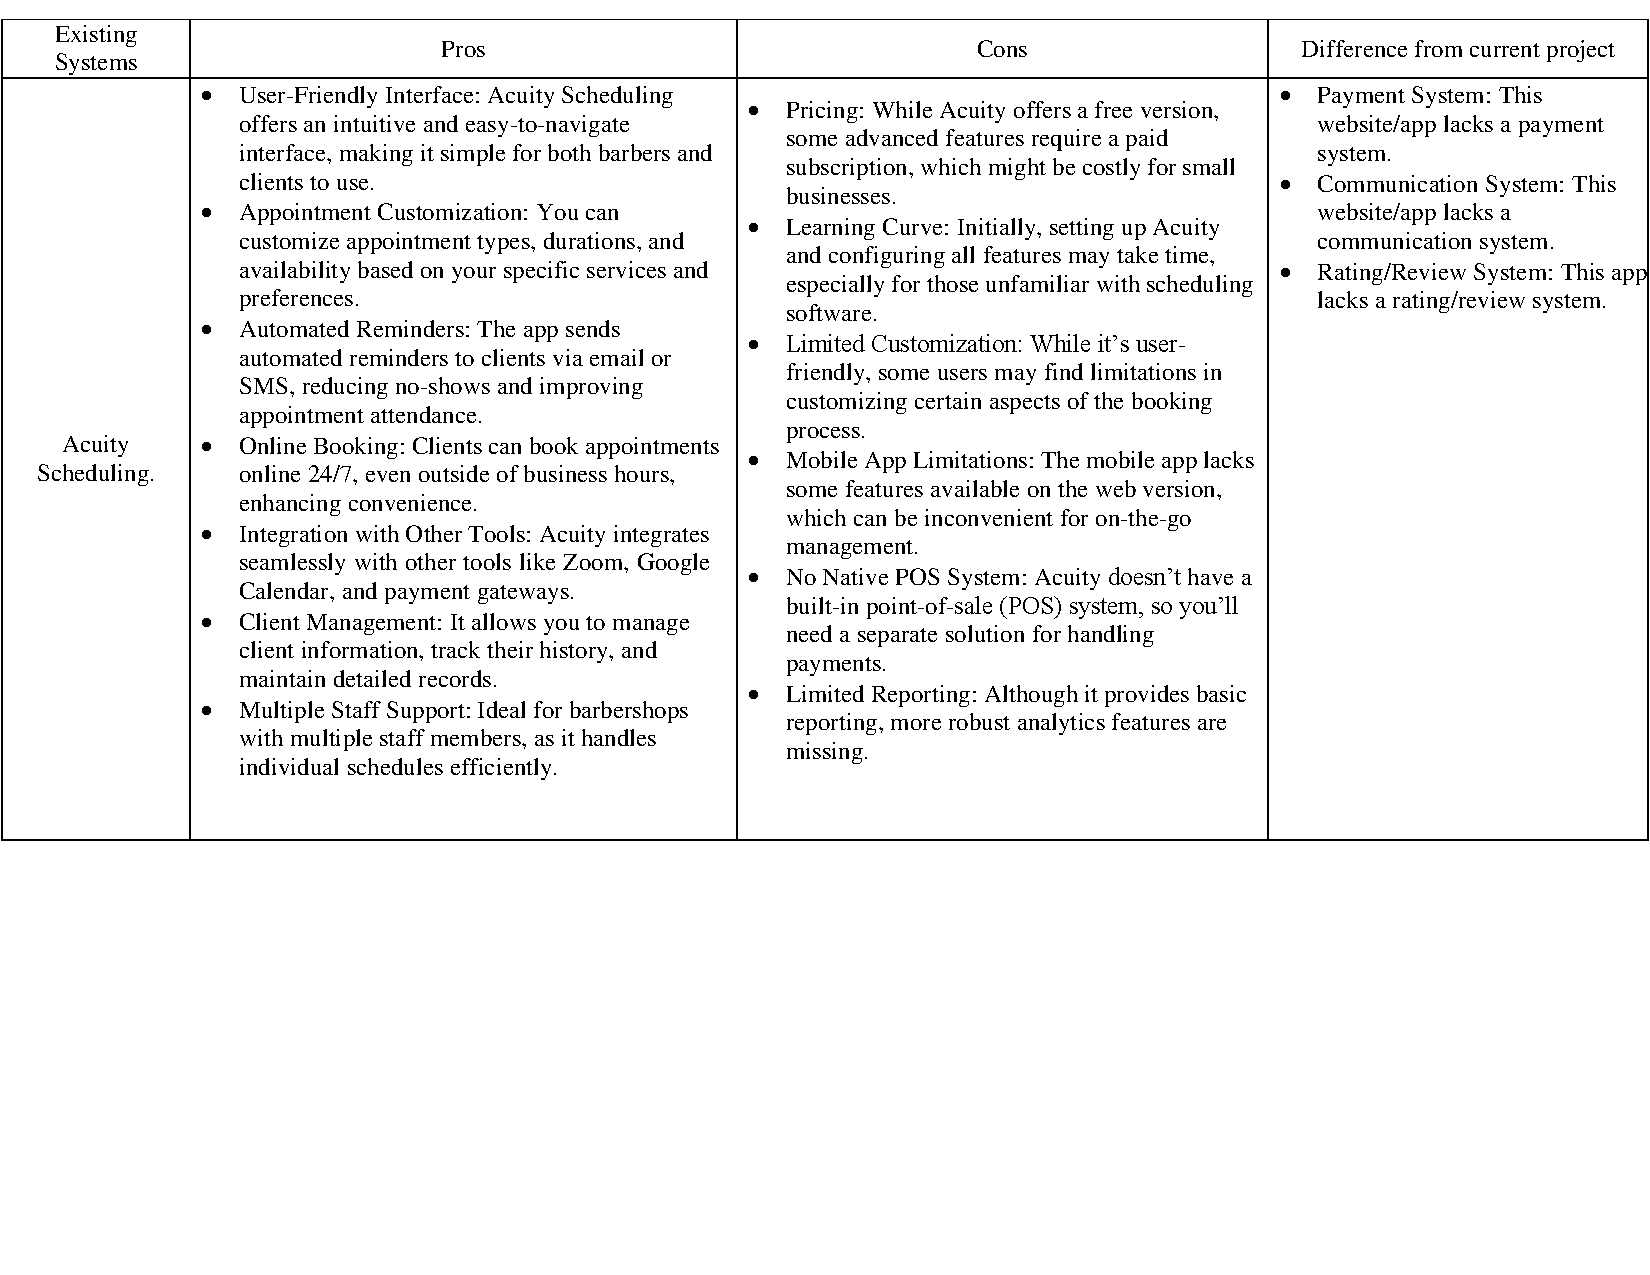
\includepdf[pages={1,2}, nup=2x1]{./attachments/Comparison_Table.pdf}

      % Include all pages of the PDF
      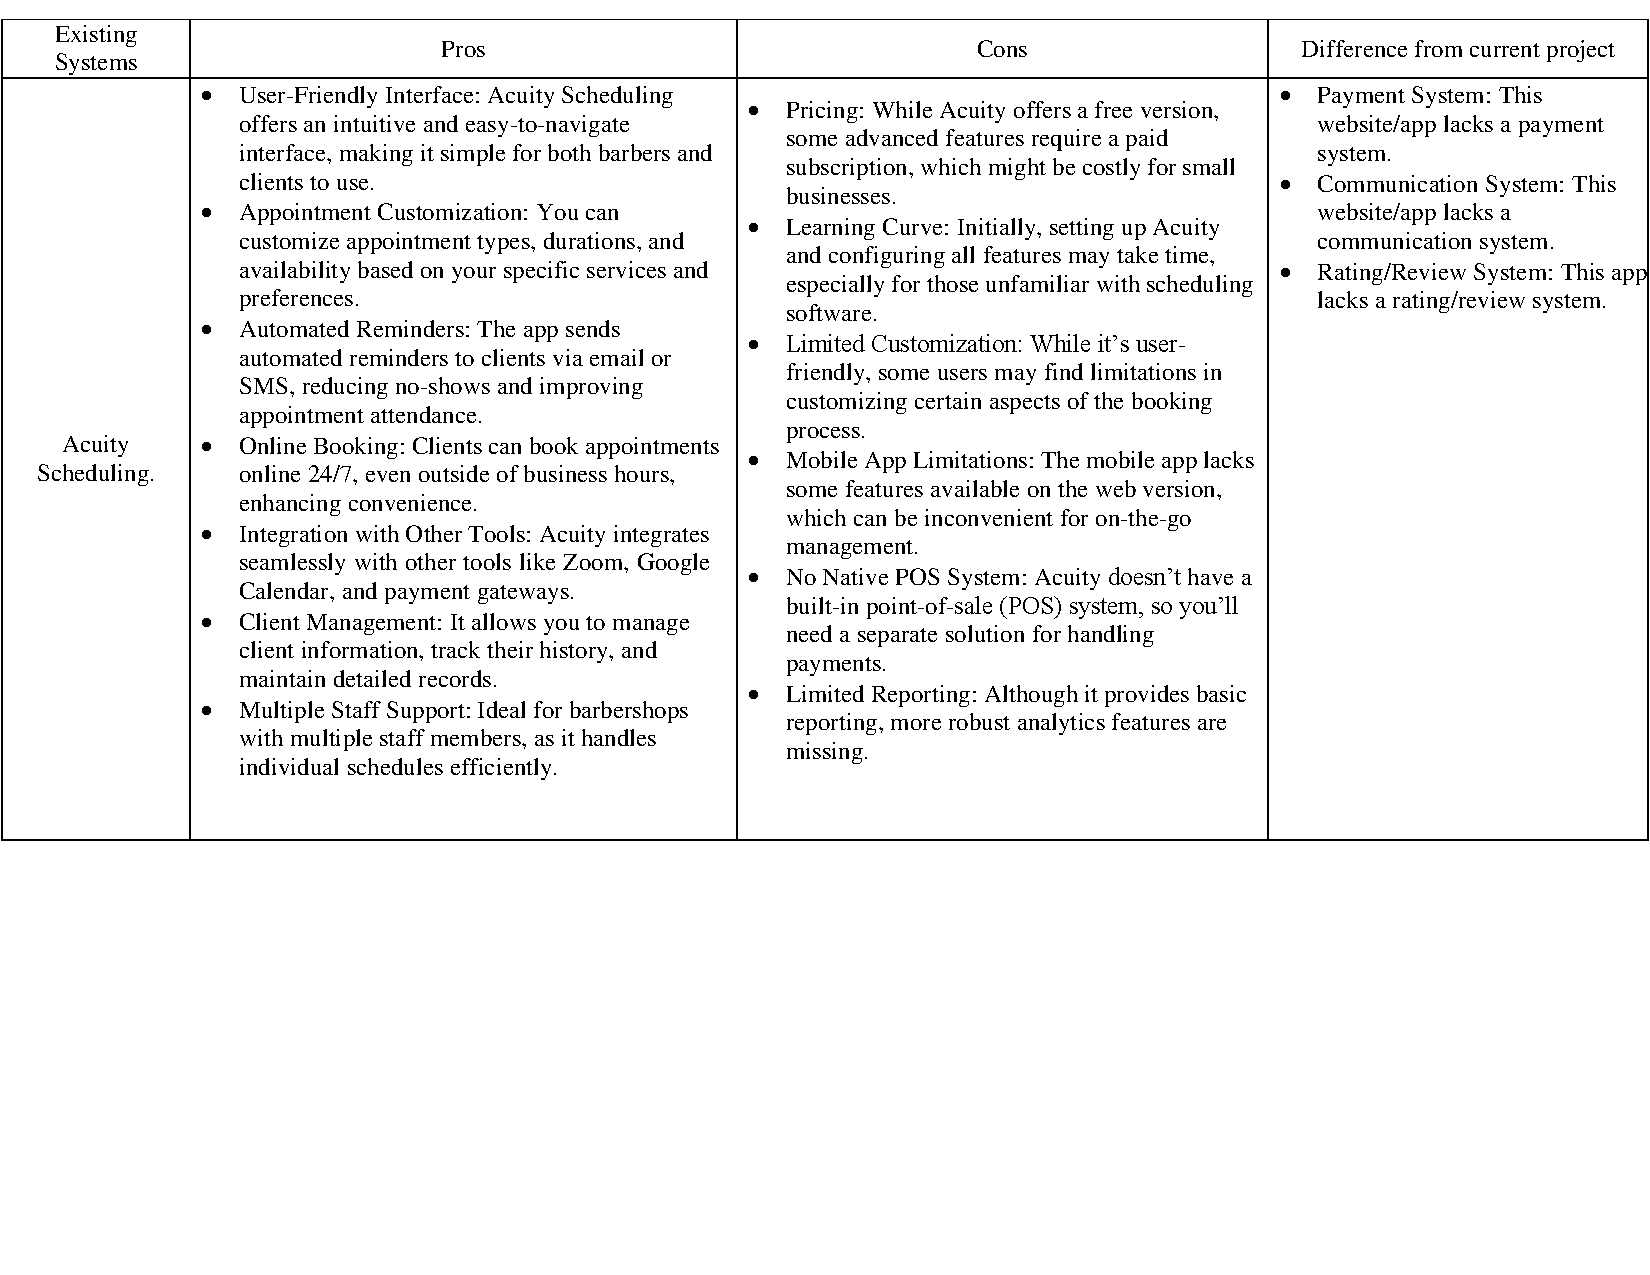
\includepdf[pages=-, fitpaper=true]{./attachments/Comparison_Table.pdf} 
      \subsection{Conclusion}
      In conclusion, this chapter summarizes the related works that are related to our project, starting with the background, and how the app would help all domains concerned with this project, starting from the customer all the way to the supplier, and detailing the literature review, existing systems and the comparisons of the pros and cons of each existing system. This chapter is the starting point for how the following chapters would take shape.

      \section{Chapter 3: General Analysis}
      \subsection{Introduction:}
      In this chapter we are going to talk about the general analysis of the application, we are going to go into detail on how we did the requirements gathering, how we define the functional and functional requirements, a display of the use case diagram, and finally a display of the dynamic diagram, in this case an activity diagram.
      
      \subsection{Requirements Gathering}
      
      In this section, we used the Google Forum method to collect questions and gather requirements related to the system, customer, barber, and admin, including functional and non-functional requirements.\newline  
    \textbf{Requirement gathering is essential for several reasons:}
    \begin{enumerate}
        \item Understanding User Needs.
        \item Scope Definition: Requirement gathering helps define the scope of the project by identifying the features.
        \item Minimizing Errors: By gathering comprehensive requirements upfront.
        \item Prioritization: It helps prioritize features and functionalities based on their importance and impact on the user experience.  
    \end{enumerate}
      \begin{figure}[htbp!]
          \centering
          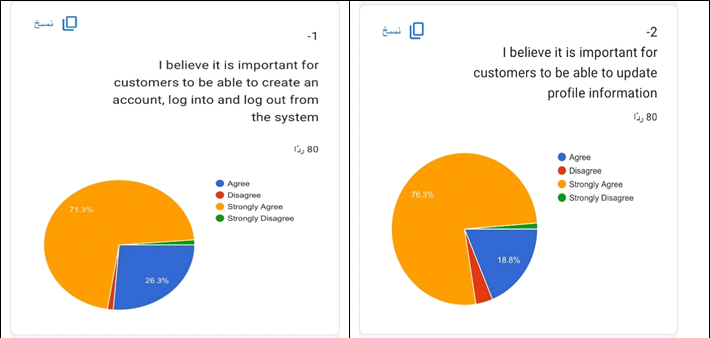
\includegraphics[width=0.80\linewidth]{images/gform1.png}
          \caption{Q1\&2}
      \end{figure}
    \textbf{1st form:} Customers can customise their experience by saving preferences, viewing, we found that most replies strongly agree on this feature.\newline
    \textbf{2nd form:} Customers can ensure that their contact details and address are correct and up to date, we found that most replies strongly agree on this feature.
      \begin{figure}[H]
          \centering
          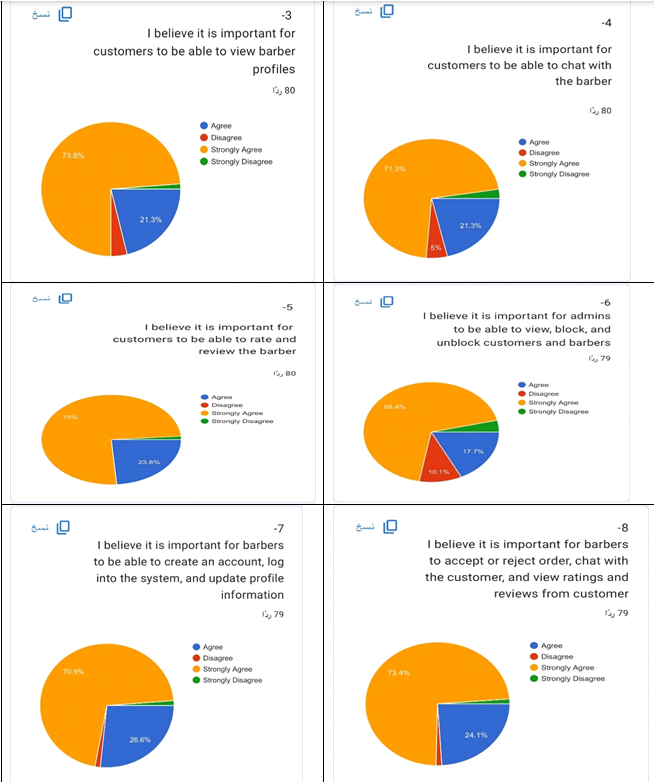
\includegraphics[width=0.80\linewidth]{images/gform2.png}
          \caption{Q3-Q8}
      \end{figure}
    \textbf{3rd form:} Customers can learn about the qualifications, experience, and specialties of individual barbers. We found that most replies strongly agree on this feature.\newline
    \textbf{4th form:} Customers can communicate their preferences, expectations, and any specific requirements directly to the barber. We found that most replies strongly agree on this feature.\newline
    \textbf{5th form: } A platform for rating and reviewing barbers creates a sense of community among customers. We found that most replies strongly agree on this feature.\newline
    \textbf{6th form: } Admins can monitor user activity and intervene if necessary to maintain a positive environment within the platform. W were mixed replies, where the majority strongly agrees on this feature, while the minority disagrees on his feature.\newline
    \textbf{7th form:} Barbers can showcase their skills, experience, and specialties through their profiles, attracting potential customers and expanding their client base. We found that most replies strongly agree on this feature.\newline
    \textbf{8th form: } Chatting with customers allows barbers to clarify any questions, discuss haircut preferences, and provide personalized recommendations. We found that most replies strongly agree on this feature.  
    \begin{figure}[H]
        \centering
        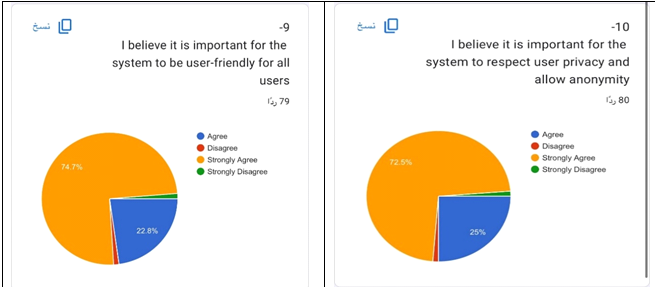
\includegraphics[width=0.80\linewidth]{images/gform3.png}
        \caption{Q9\&10}
    \end{figure} 
    \textbf{9th form:} A user-friendly interface ensures that individuals of all abilities can navigate and interact with the system easily, promoting inclusivity and equal access to services. We found that most replies strongly agree on this feature.\newline
    \textbf{10th form:} When users feel confident that their privacy is respected and their identity remains anonymous, they are more likely to trust the platform with their personal information and engage more freely. We found that most replies strongly agree on this feature.
    
       \subsection{Functional Requirements}
      
      In this section, we are going to list the functional requirements that the system needs to function properly, starting with the customer functionality, barber functionality, and finally the admin functionality.
      
      For the \textbf{Customer} functionality we have the following requirements:
      \begin{itemize}
        \item The customer shall be able to create an account in the system.
        \item The customer shall be able to log into the system.
        \item The customer shall be able to renew the forgotten password.
        \item The customer shall be able to update profile information.
        \item The customer shall be able to View Barber Profiles. 
        \item The customer shall be able to send orders of appointments to the barber. 
        \item The customer shall be able to chat with the barber. 
        \item The customer shall be able to rate and review the barber.
        \item The customer shall be able to make payments to the barber.
        \item The customer shall be able to log out of the system.  
      \end{itemize}      
       As for the \textbf{Barber} functionality we have the following requirements:
       \begin{itemize}
        \item The barber shall be able to create an account in the system.
        \item The barber shall be able to log in to the system. 
        \item The barber shall be able to reset the password.
        \item The barber shall be able to update profile information.
        \item The barber shall be able to receive orders of appointments from customers. 
        \item The barber shall be able to accept or reject the orders.
        \item The barber shall be able to chat with the customer. 
        \item The barber shall be able to view ratings and reviews from customers and rate the customers.
        \item The barber shall be able to log out of the system.
       \end{itemize}\pagebreak
       And finally, for the \textbf{admin} functionality we have the following requirements:
       \begin{itemize}
        \item The admin shall be able to log in to the system.
        \item The admin shall be able to reset forgotten password. 
        \item The admin shall be able to view, block, and unblock customers.
        \item The admin shall be able to view, block, and unblock barbers. 
        \item The admin shall be able to view and delete reviews and ratings. 
        \item The admin shall log out from the system.
       \end{itemize}      
      \subsection{Non-functional Requirements}
      In this section, we are going to list the non-functional requirements that are expected to be in the system, and those non-functional requirements are:
      \begin{itemize}
        \item User friendly: The system will be giving a very user-friendly approach for all users.
        \item Flexible: Can change the setting - Availability: 24 hours available.
        \item Accessibility: The phone is accessible to almost everyone and access to the app is also easy. 
        \item Performance: Response times, processing times, query, and reporting times.
        \item Easy maintenance: The app is designed easily, so maintenance is also easy.
        \item Security: The application protects sensitive user information (such as a password).
        \item Privacy: The user does not want to show his identity.
      \end{itemize}
      \subsection{Use Case Diagram}
       In this section, we are going to display the use case diagram that reflects the functional requirements of the system, starting with the customer functionality, barber functionality and finally the admin functionality.
            \begin{figure}[H]
                \centering
                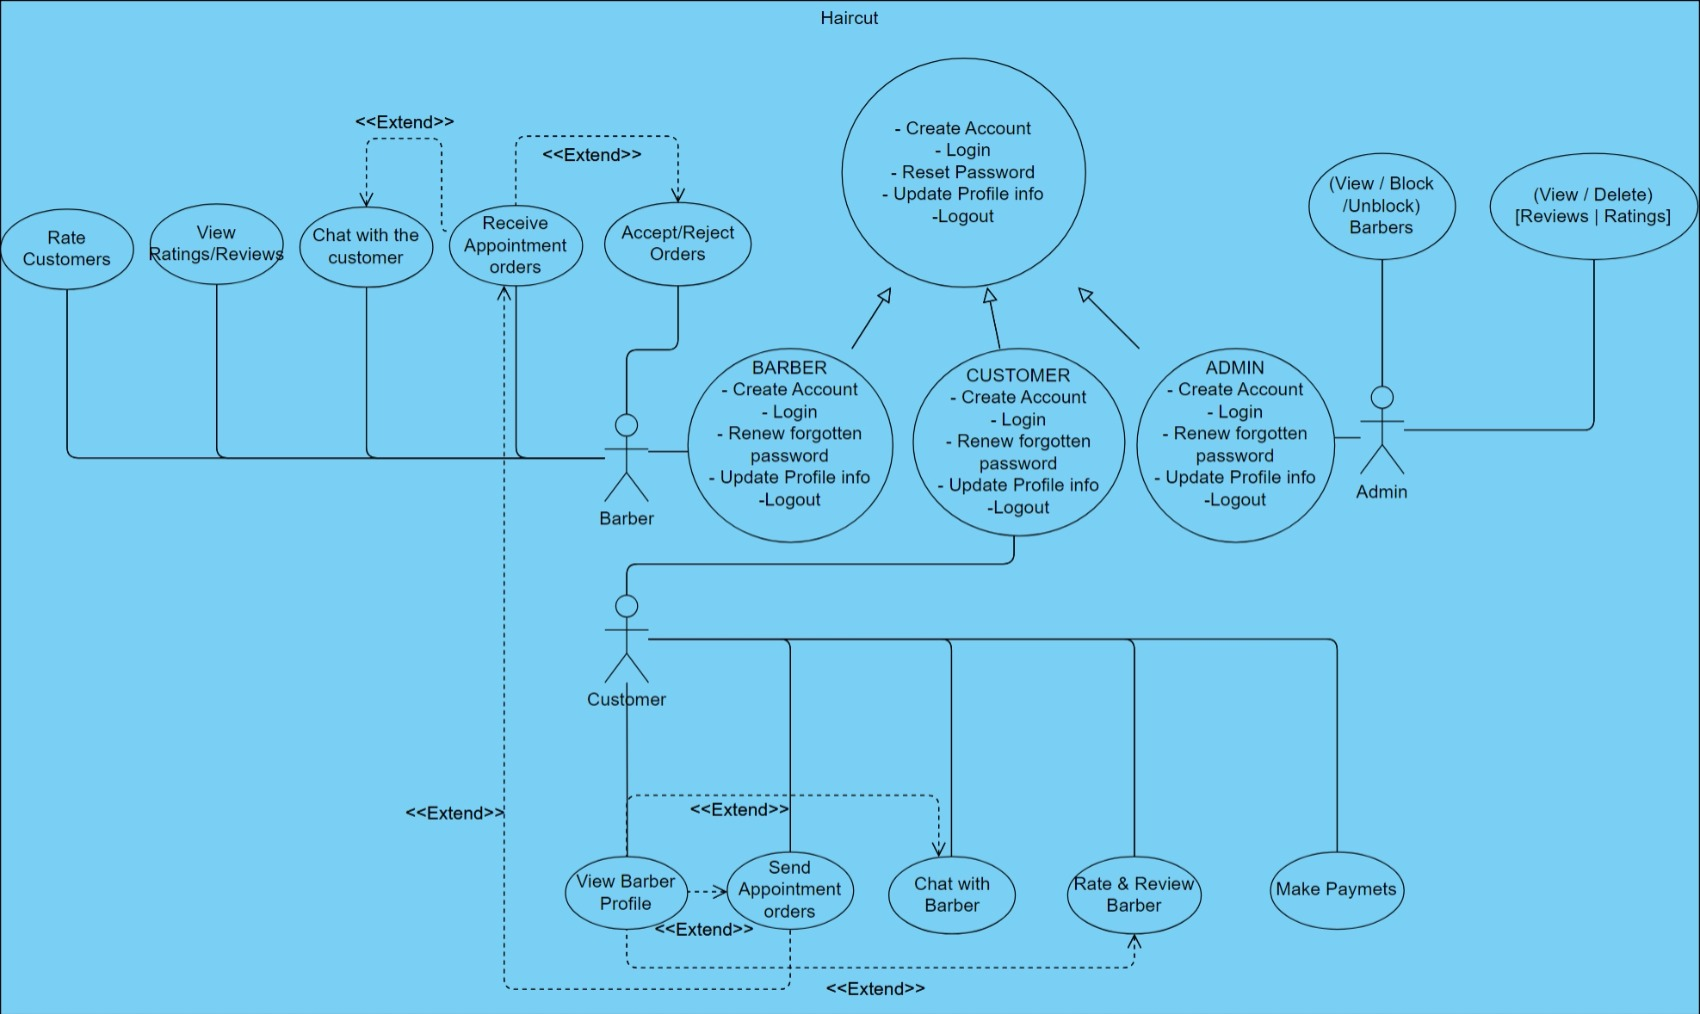
\includegraphics[width=1\linewidth]{images/Use_case_diagram.jpg}
                \caption{Use Case Diagram}
            \end{figure}
      \subsection{Dynamic Diagram}
       In this section, we are going to display the general dynamic diagram to display how the system works, in this case we chose an activity diagram, which showcases the steps of the system, starting from the customer log in, sending an order of appointment, if it's accepted, then the appointment is booked, receiving the service, making the payment, either payment by cash or credit card, then finally rating/reviewing the barber. As for the barber, he logs in, receives order of appointment, either accept or reject, if rejected, he notifies the customer, if accepted, the appointment is booked, gives the service, receives the payment, then finally rating/reviewing the customer.
      \begin{figure}[H]
          \centering
          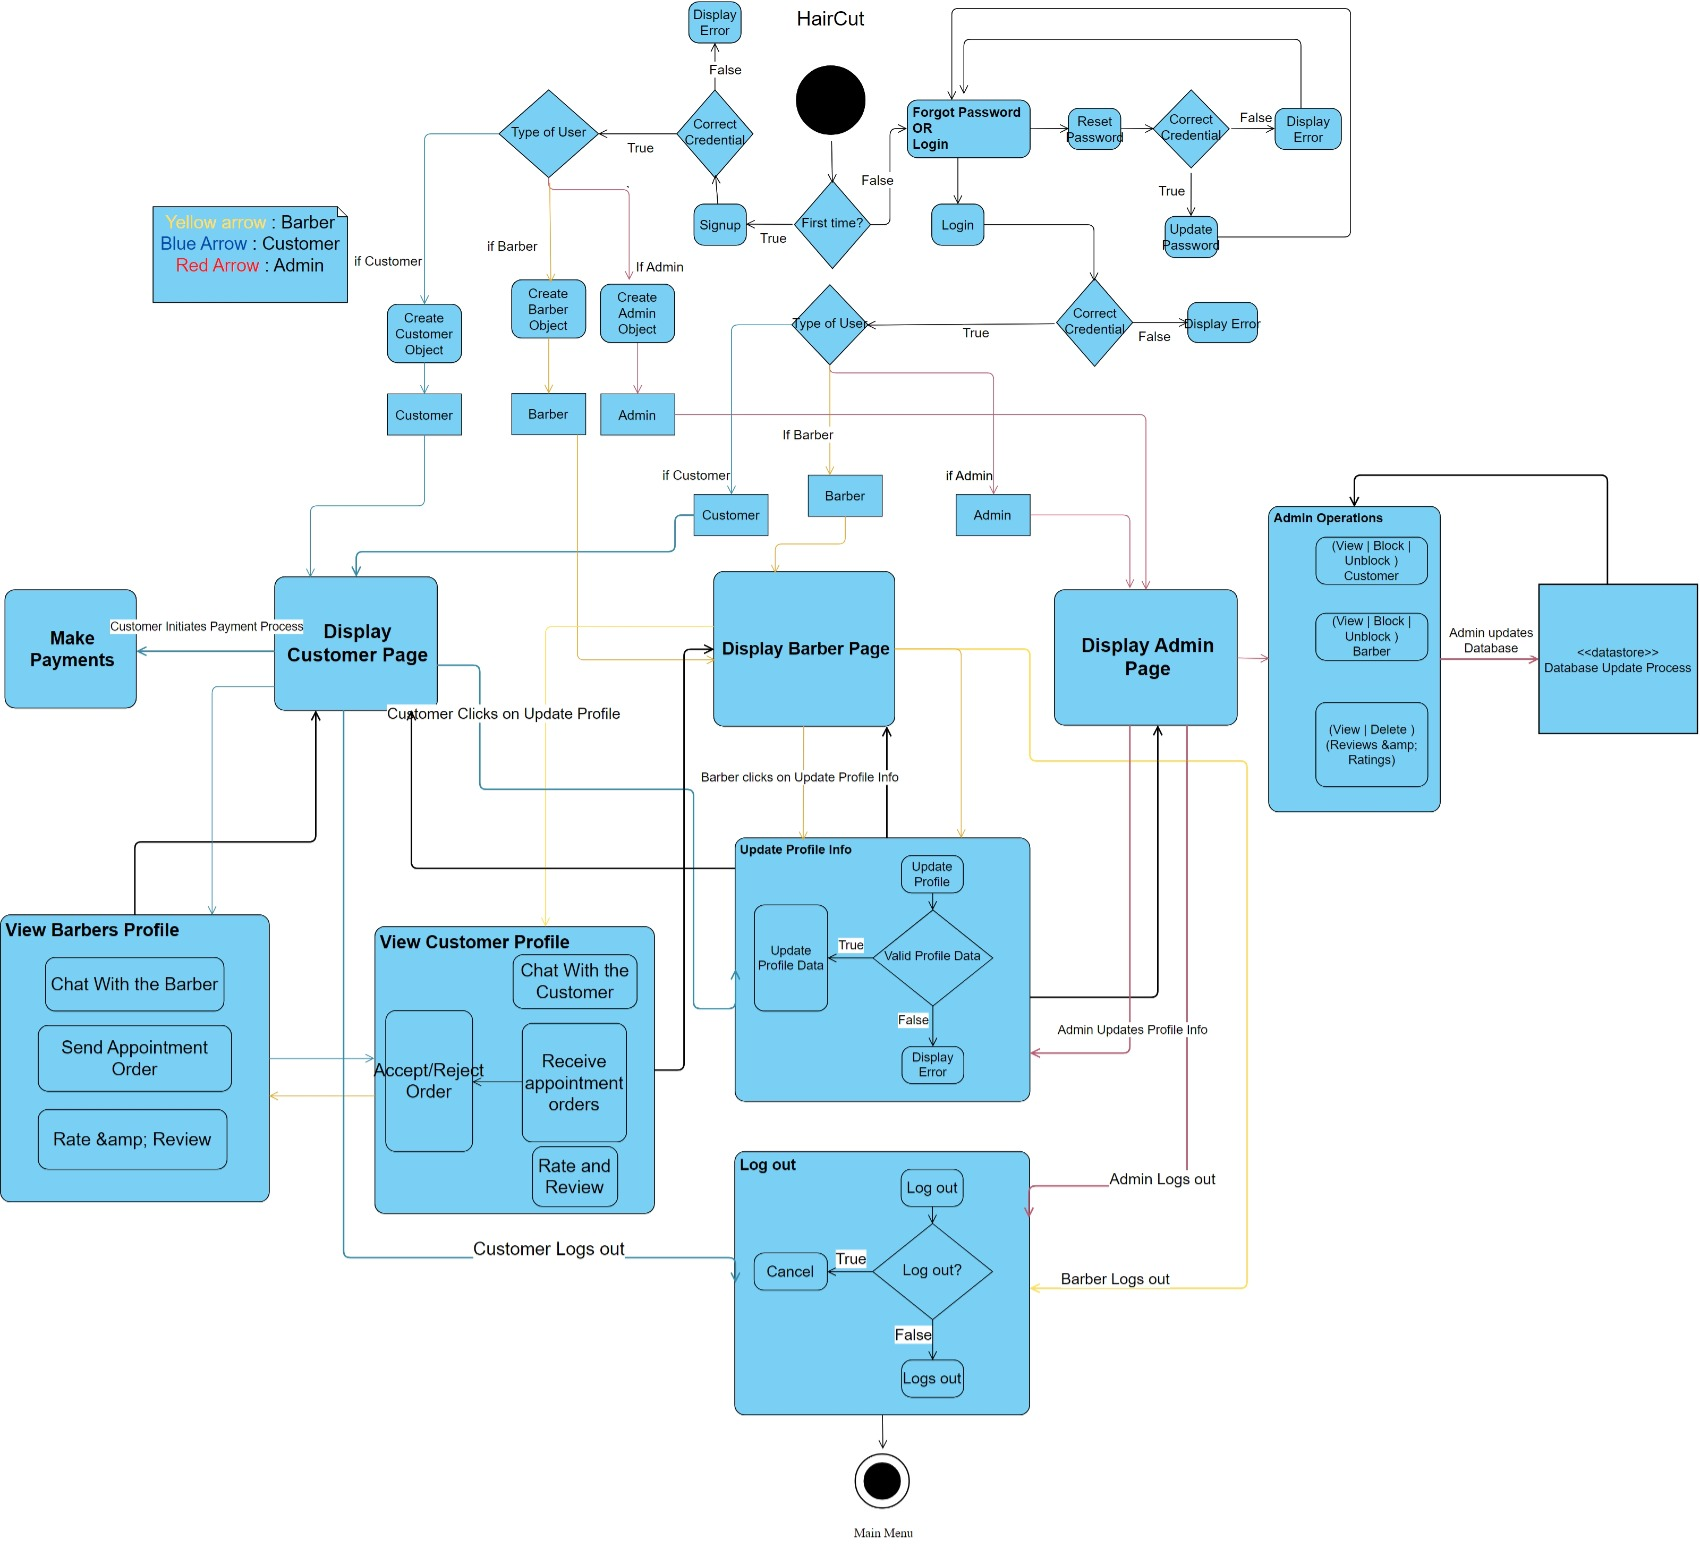
\includegraphics[width=0.75\linewidth]{images/Dynamic_activity_diagram.jpg}
          \caption{Activity Diagram}
      \end{figure}
      \subsection{Conclusion}
       In conclusion, this chapter was a general analysis of the system, and describing how we gathered requirements using the technique of google form and the statistics, listing the functional and non-functional requirements, displaying the use case diagram, and finally displaying the dynamic diagram and its description.
      \section{Chapter 4: Detailed Design}
      \subsection{Introduction}
      In this chapter we are going to discuss the detailed design of the application, discussing the static aspects of the application, the architectural aspect design of the application, the dynamic aspect design of the application, and finally, the user interface design of the application.
      \subsection{Static Aspect Design}
      
      \begin{figure}[H]
          \centering
          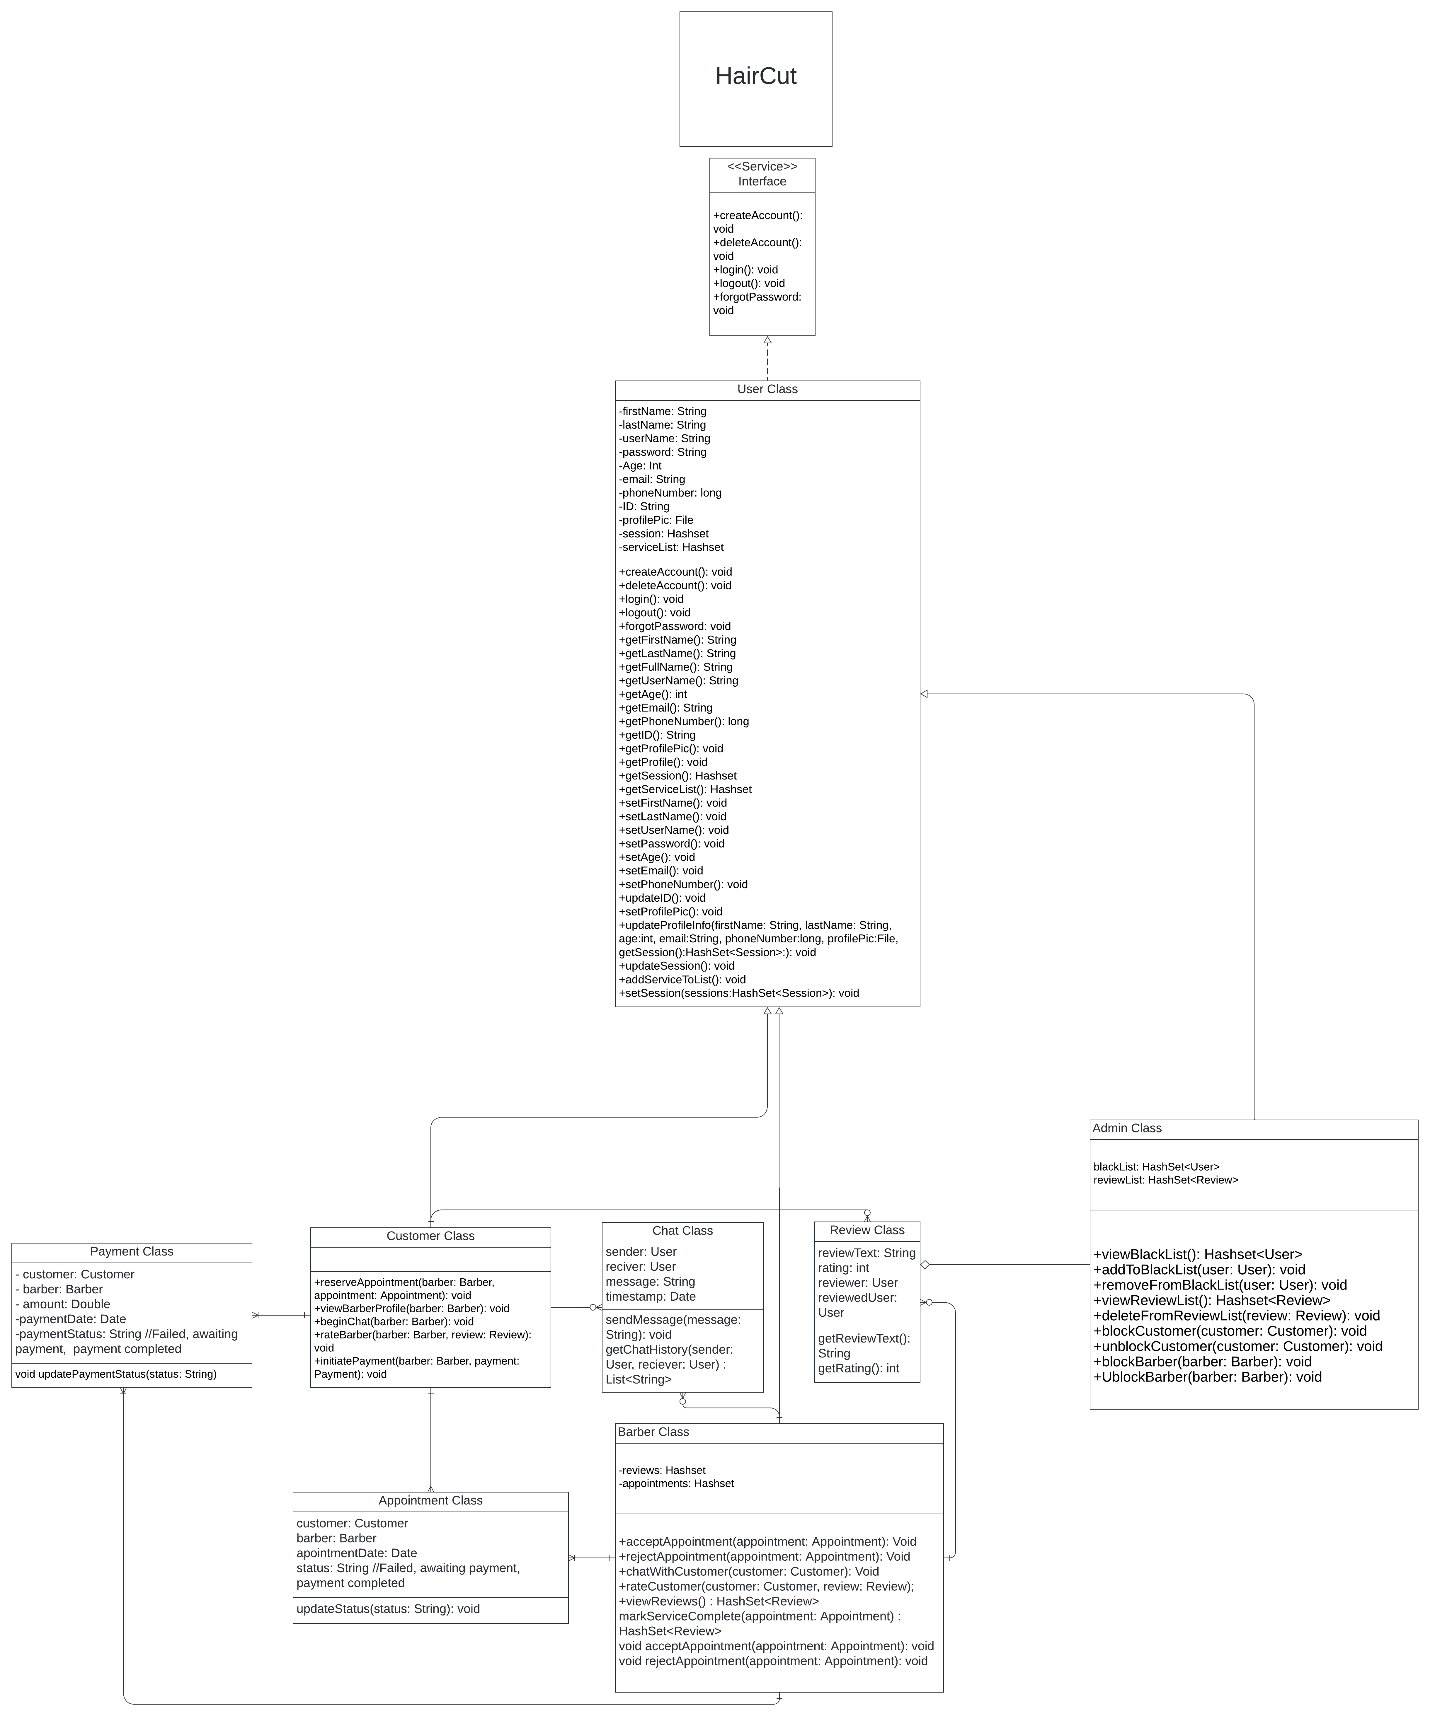
\includegraphics[width=1\linewidth]{images/class_diagram.png}
          \caption{Class Diagram}
      \end{figure}
      \subsection{Architectural Aspect Design}
      
      In general, we created the system as a mobile application, which the users will access using a mobile phone. We primarily targeted customers and barbers who would be reserving \& offering services. Customers will use the mobile application to reserve appointments and use other services, and the barbers will interact with customers, offer their services and the admin will maintain the services between the two parties.
      \begin{figure}[H]
          \centering
          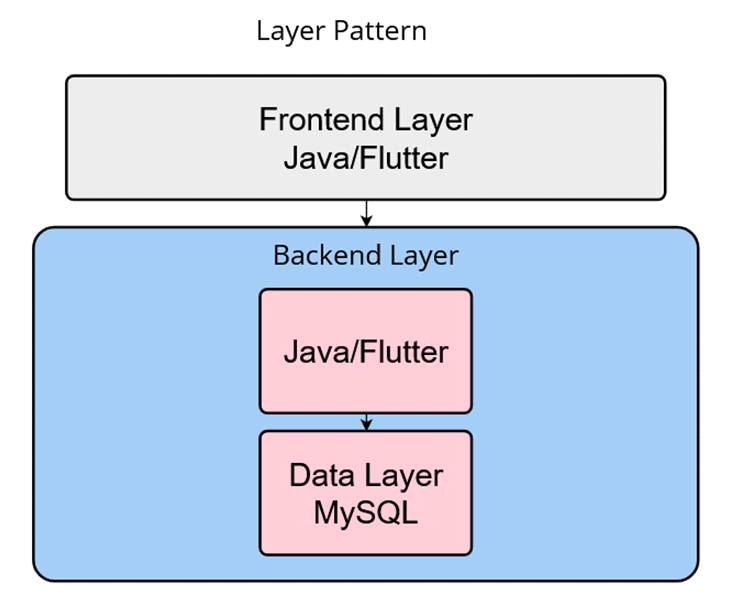
\includegraphics[width=0.75\linewidth]{images/layer pattern.png}
          \caption{Layer Pattern}
      \end{figure}
        \begin{figure}[H]
            \centering
            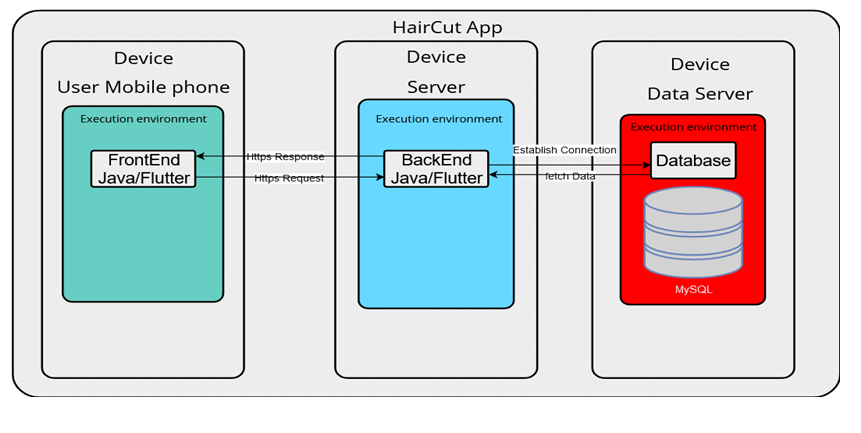
\includegraphics[width=0.75\linewidth]{images/deployment diagram.png}
            \caption{Deployment Diagram}
        \end{figure}
      \subsection{Dynamic Aspect Design}

    \begin{figure}[H]
        \centering
        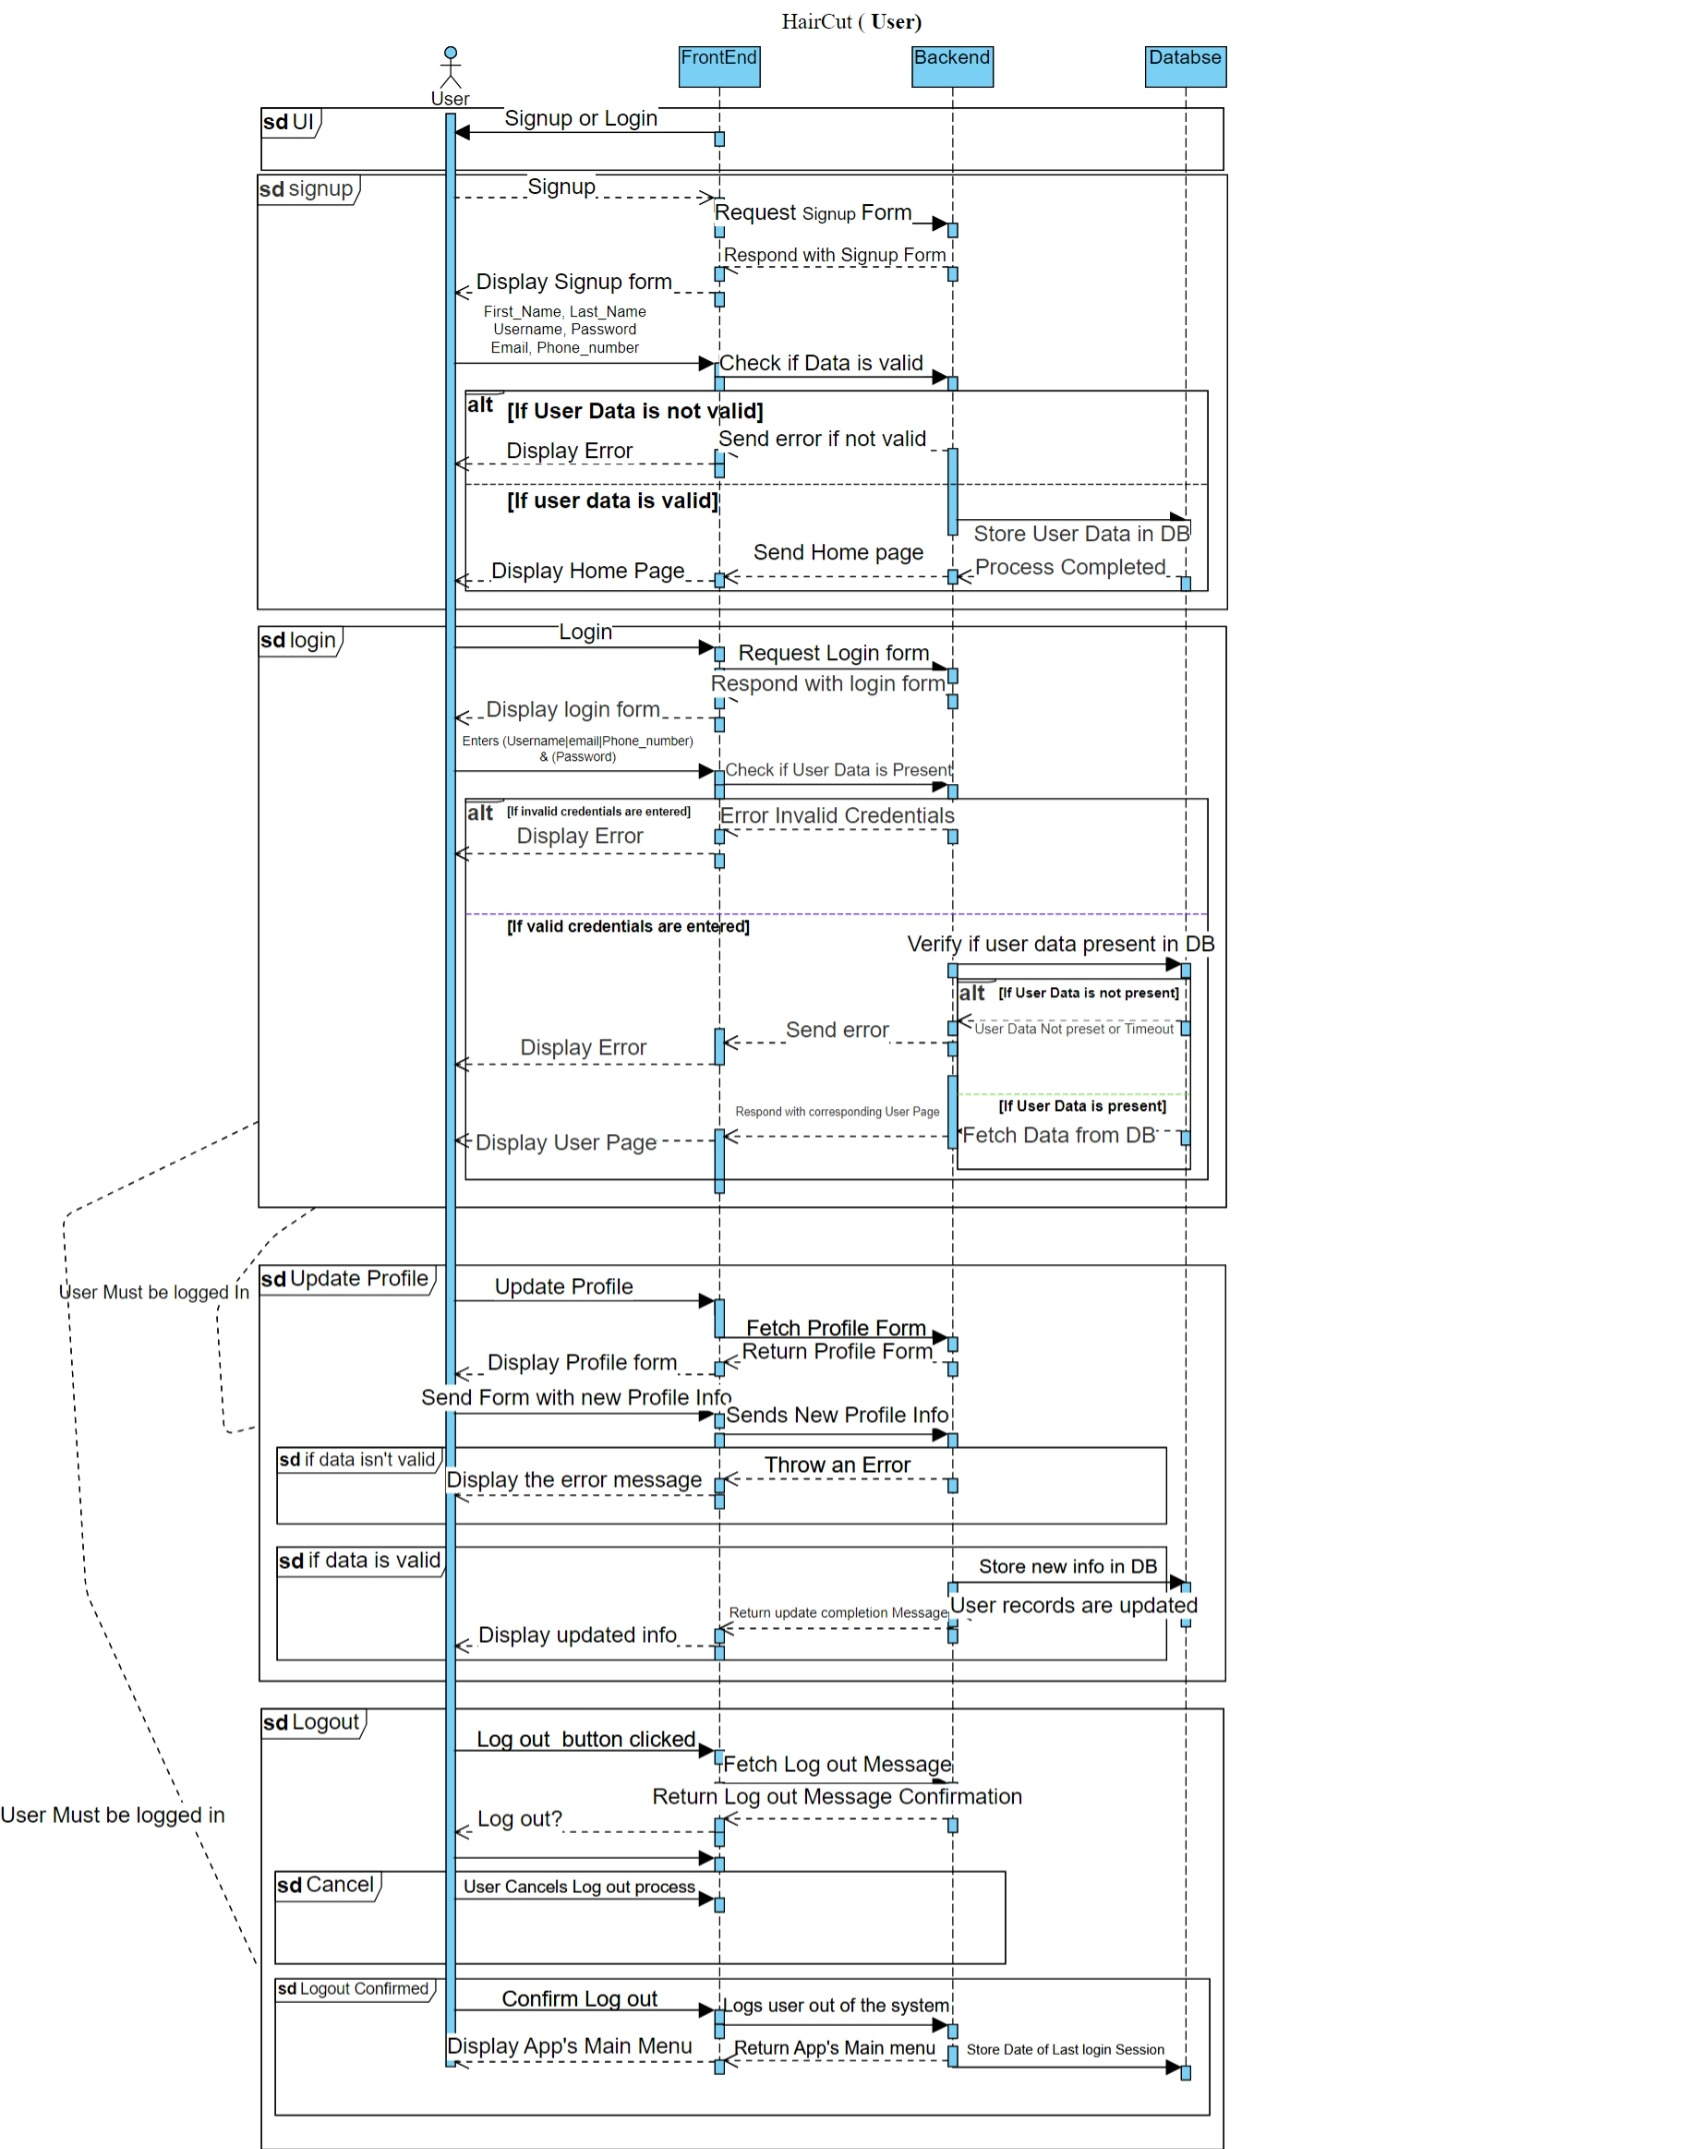
\includegraphics[width=0.75\linewidth]{images/Sequence_Diagram_1_Signup_Login_Update-Profile_Logout.jpg}
        \caption{Sequence Diagram 1: [User Diagram] sign up, login, update profile and logout}
    \end{figure}
    \begin{figure}[H]
        \centering
        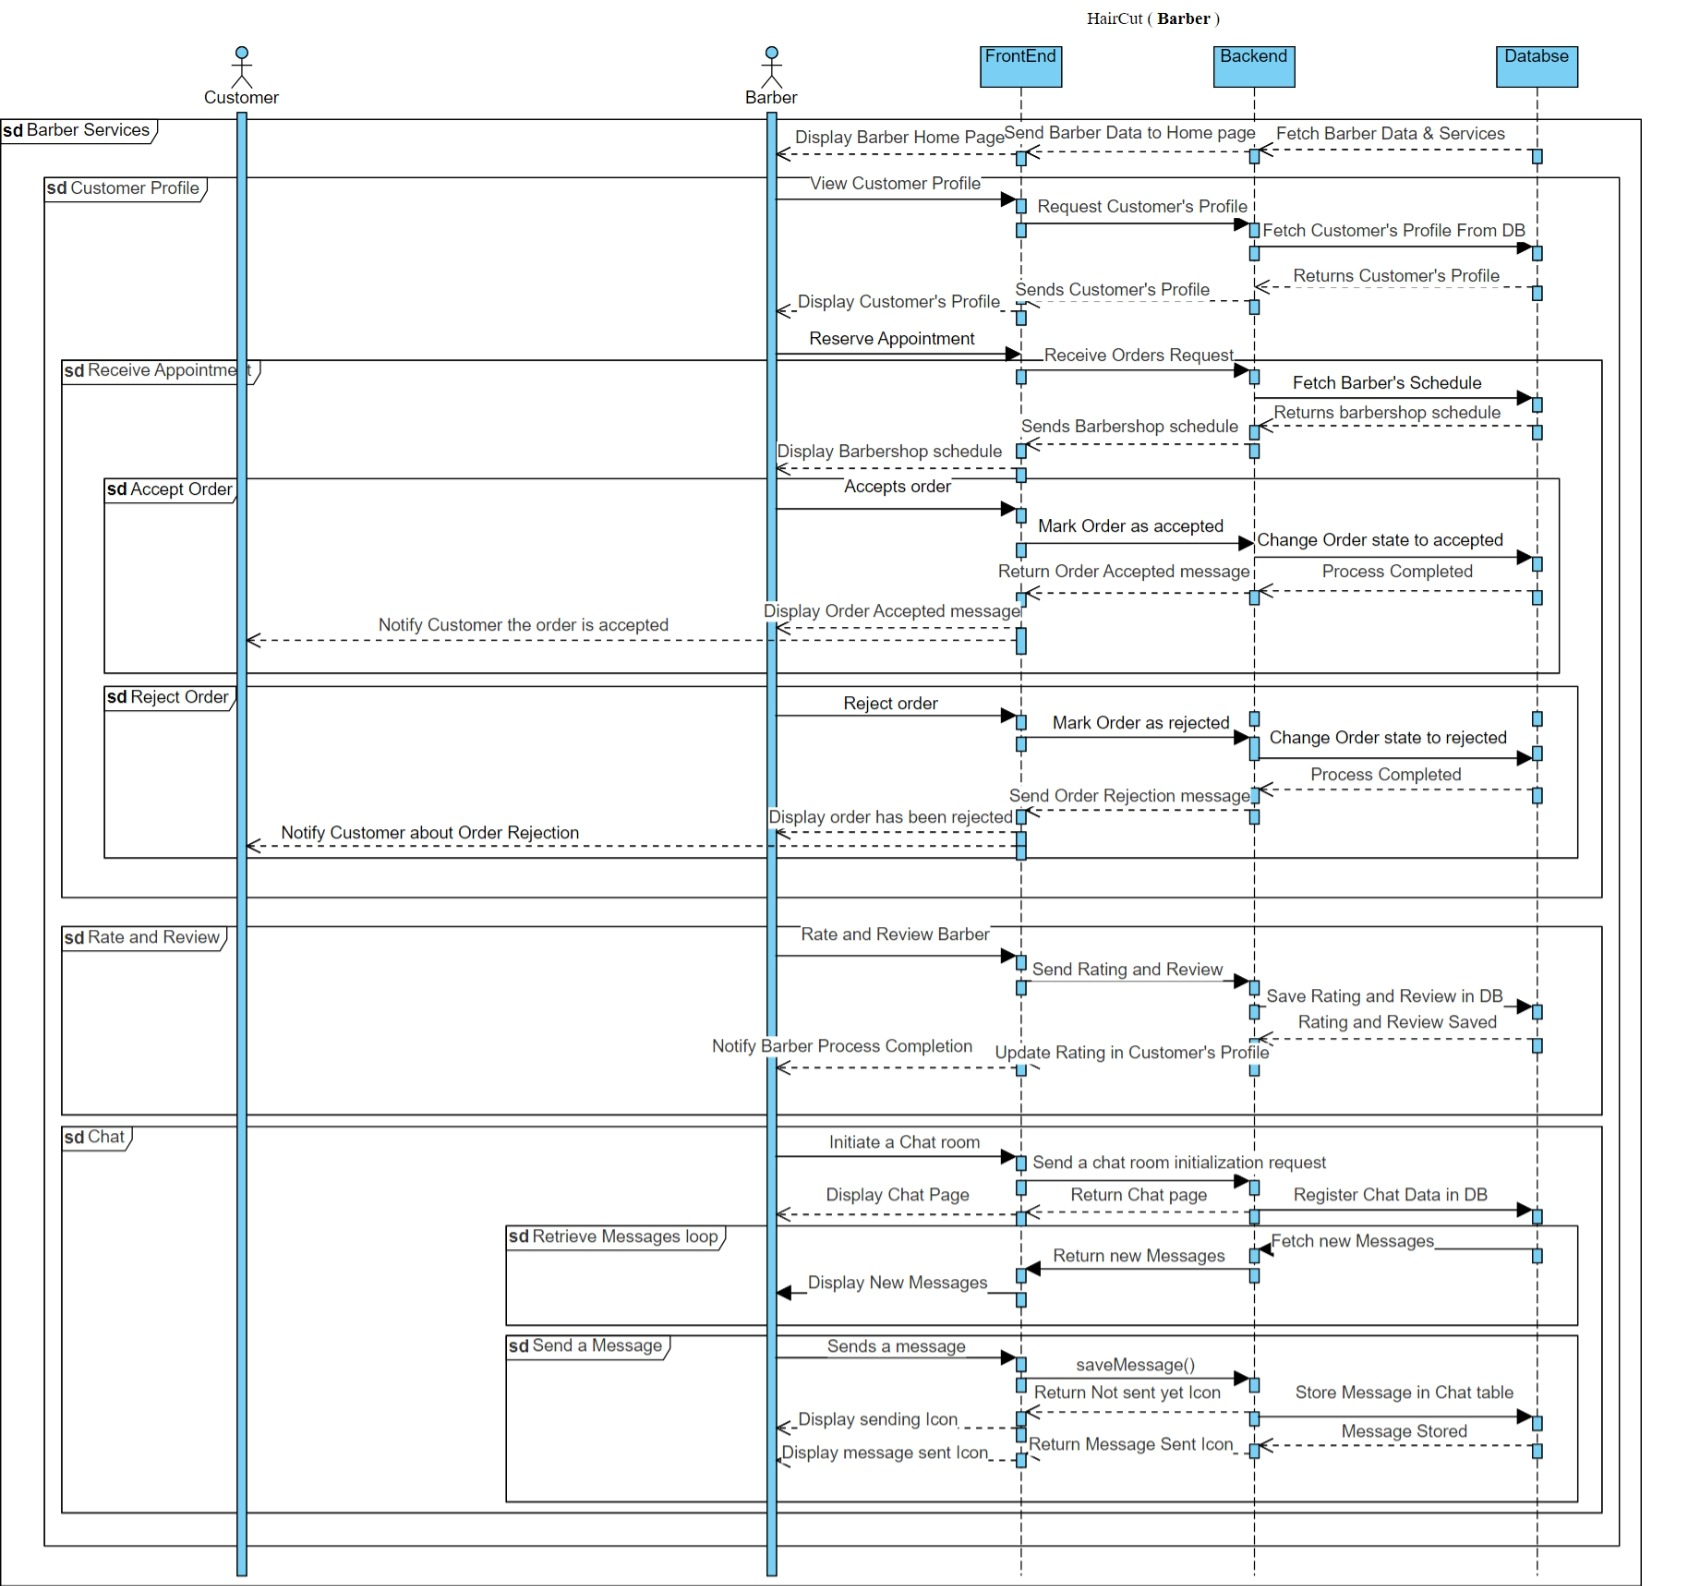
\includegraphics[width=0.75\linewidth]{images/Sequence_Diagram_2_Barber-Services.jpg}
        \caption{Sequence Diagram 2: Barber Services}
    \end{figure}
    \begin{figure}[H]
        \centering
        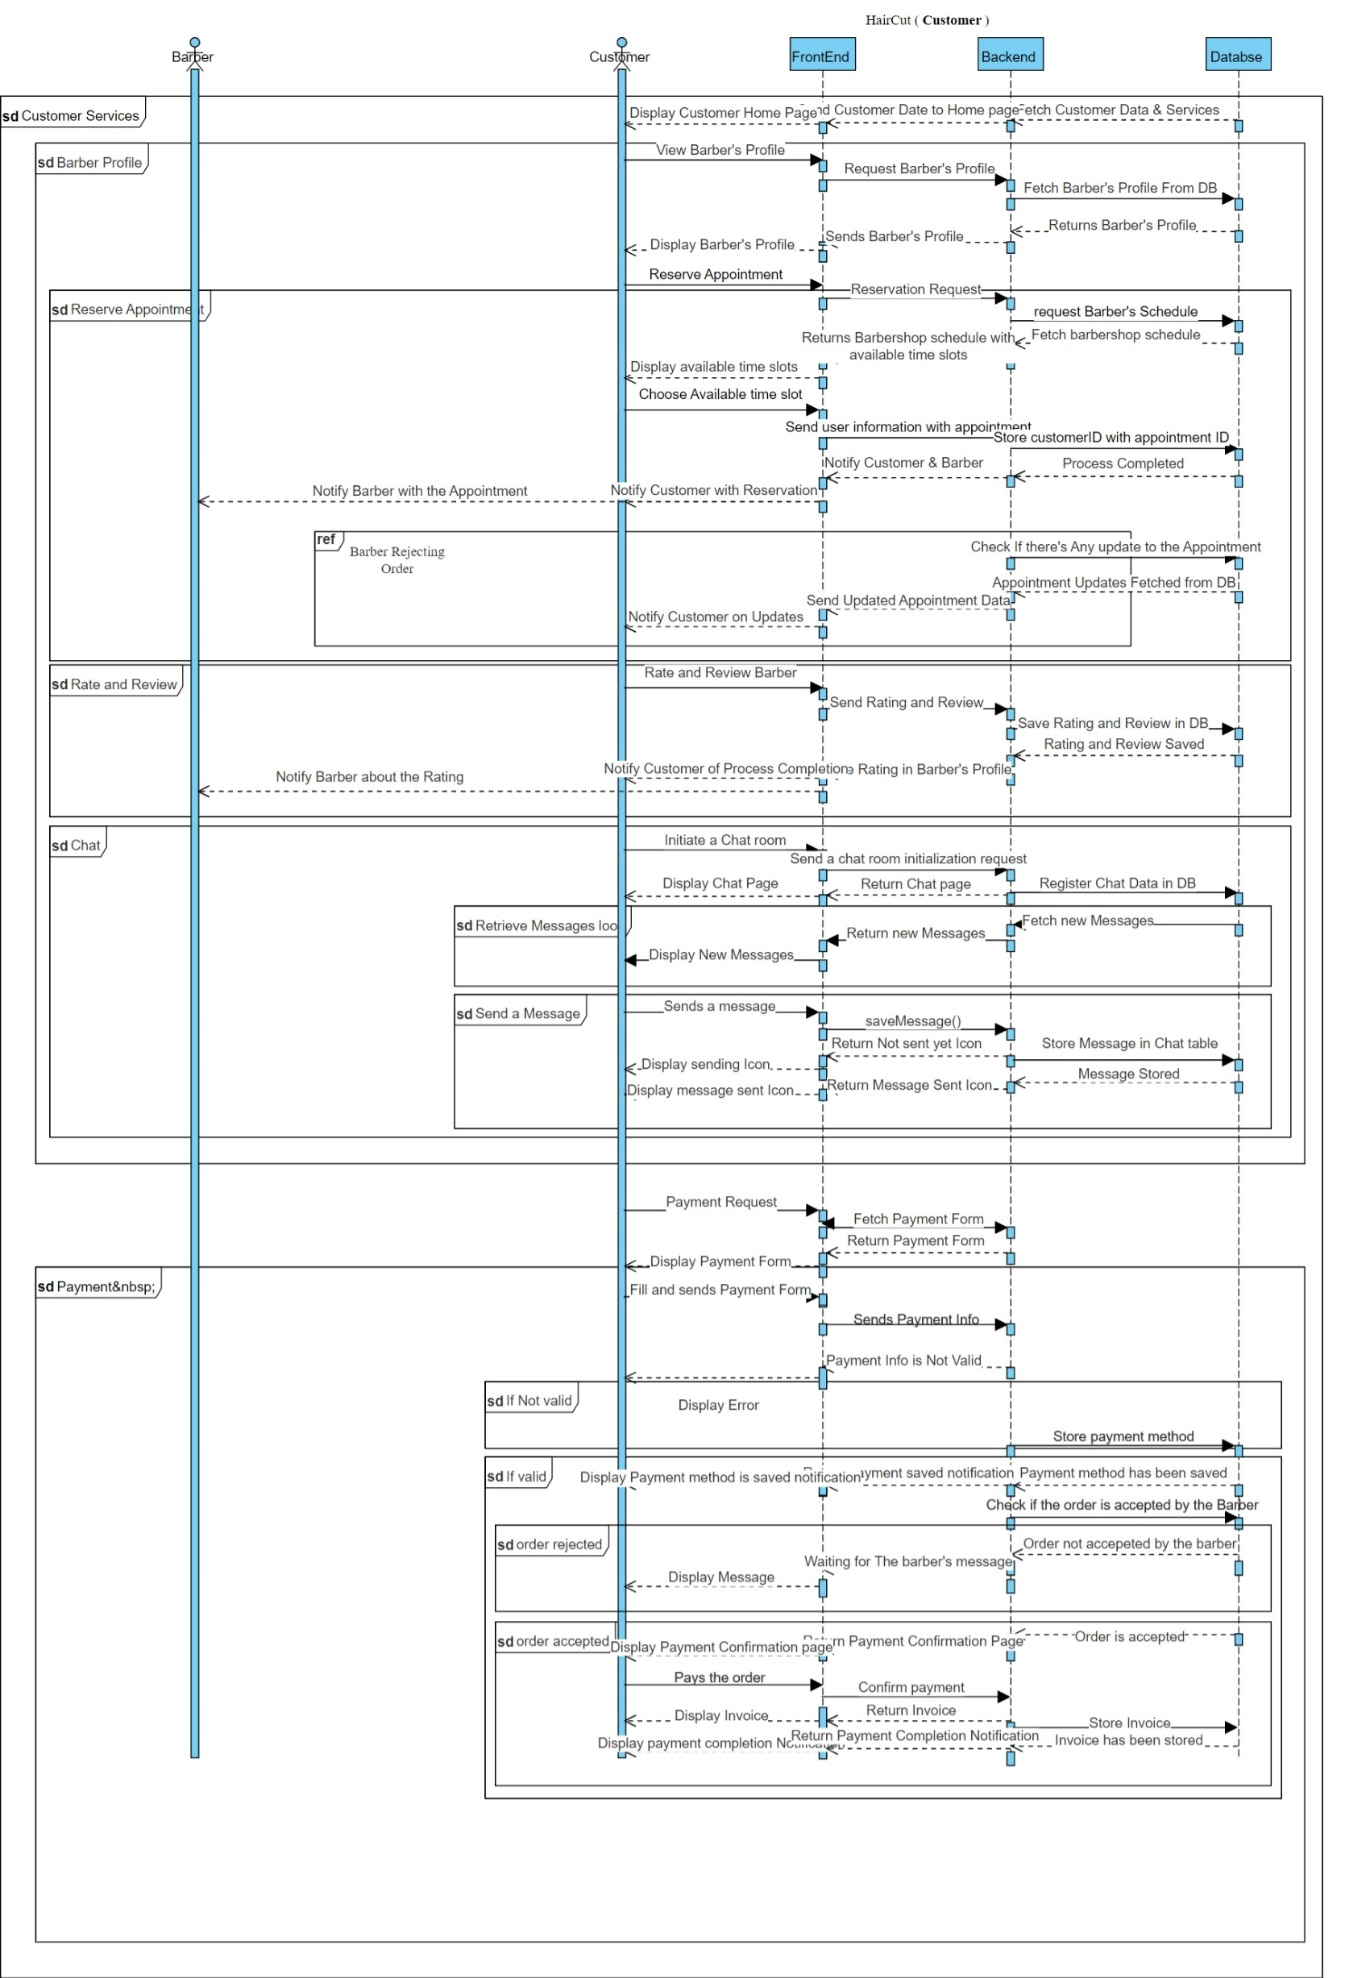
\includegraphics[width=0.75\linewidth]{images/Sequence_Diagram_3_Customer-Services.jpg}
        \caption{Sequence Diagram 3: Customer Services}
    \end{figure}
    \begin{figure}[H]
        \centering
        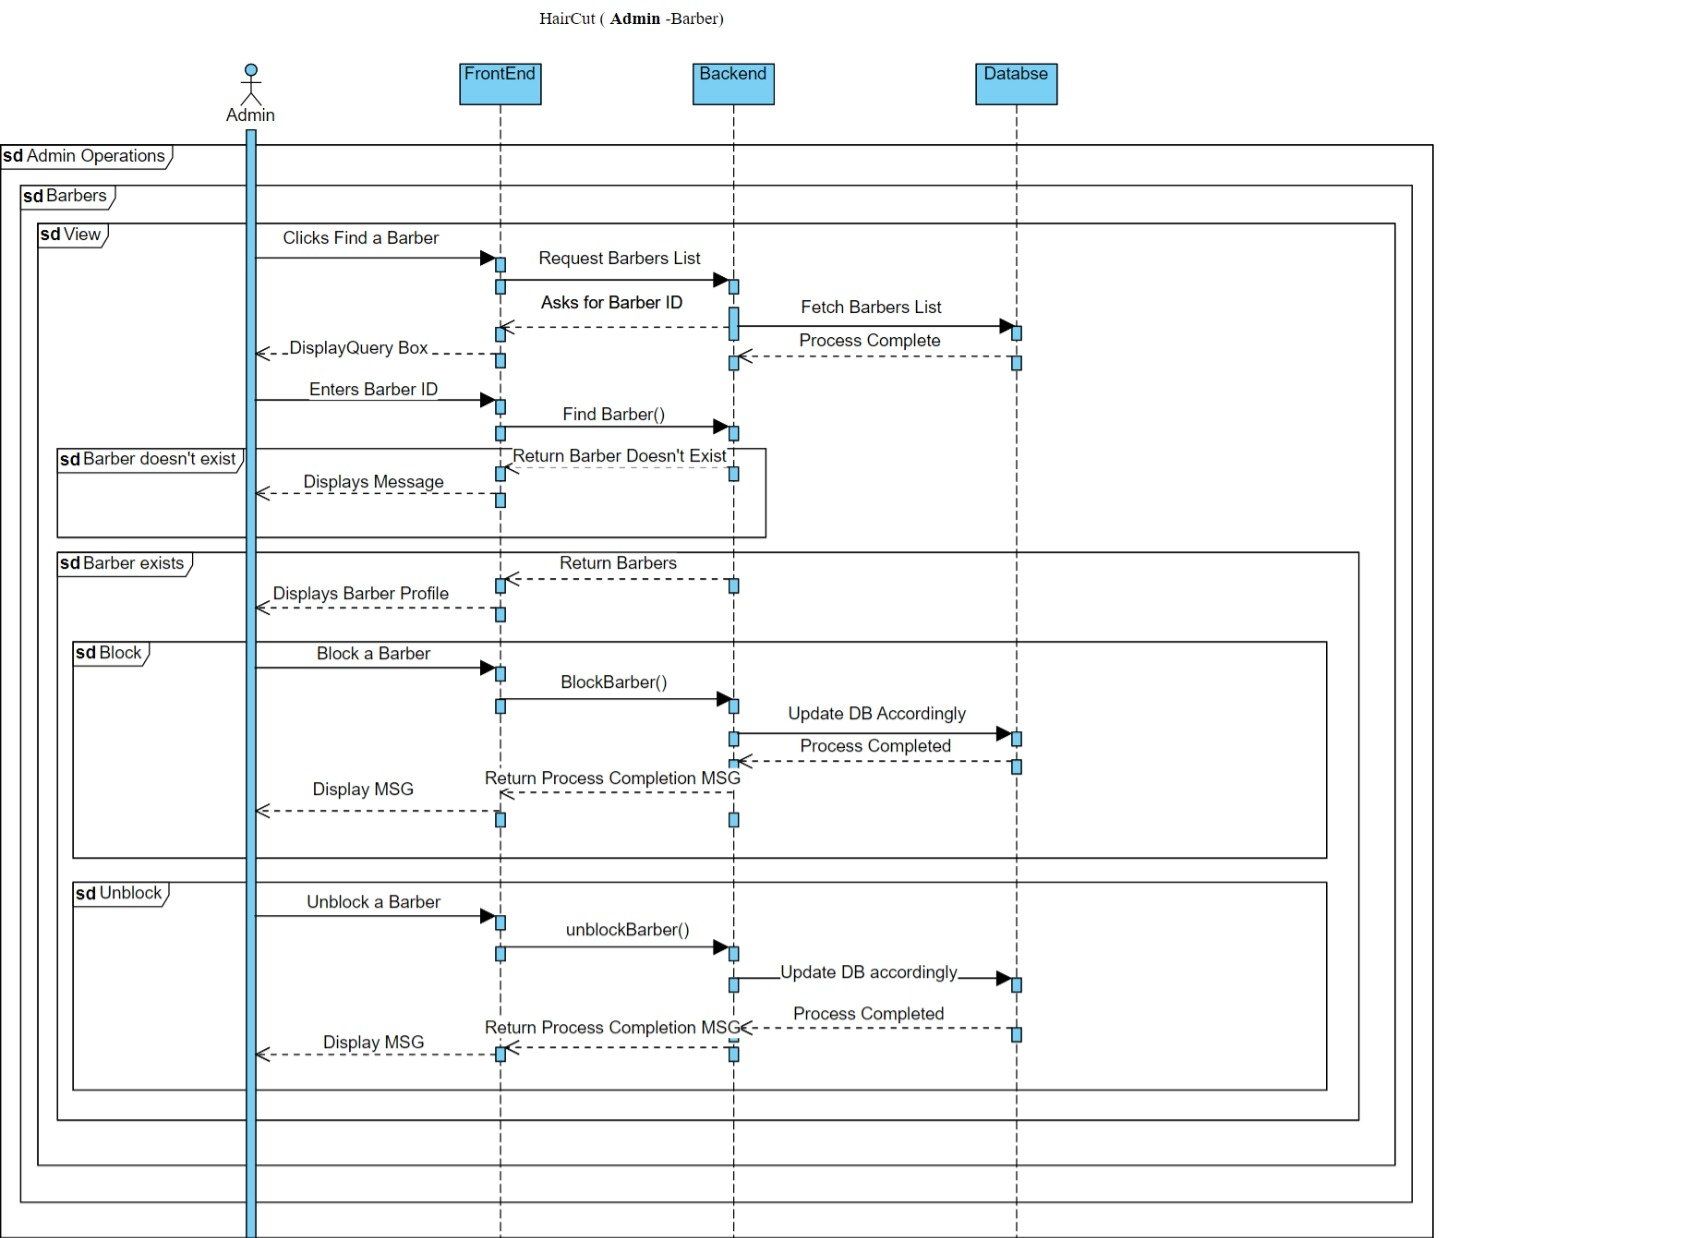
\includegraphics[width=0.75\linewidth]{images/Sequence_Diagram_4_Admin-Operations-Barbers.jpg}
        \caption{Sequence Diagram 4: [Admin Diagram 1] Admin operations on barbers}
    \end{figure}
    \begin{figure}[H]
        \centering
        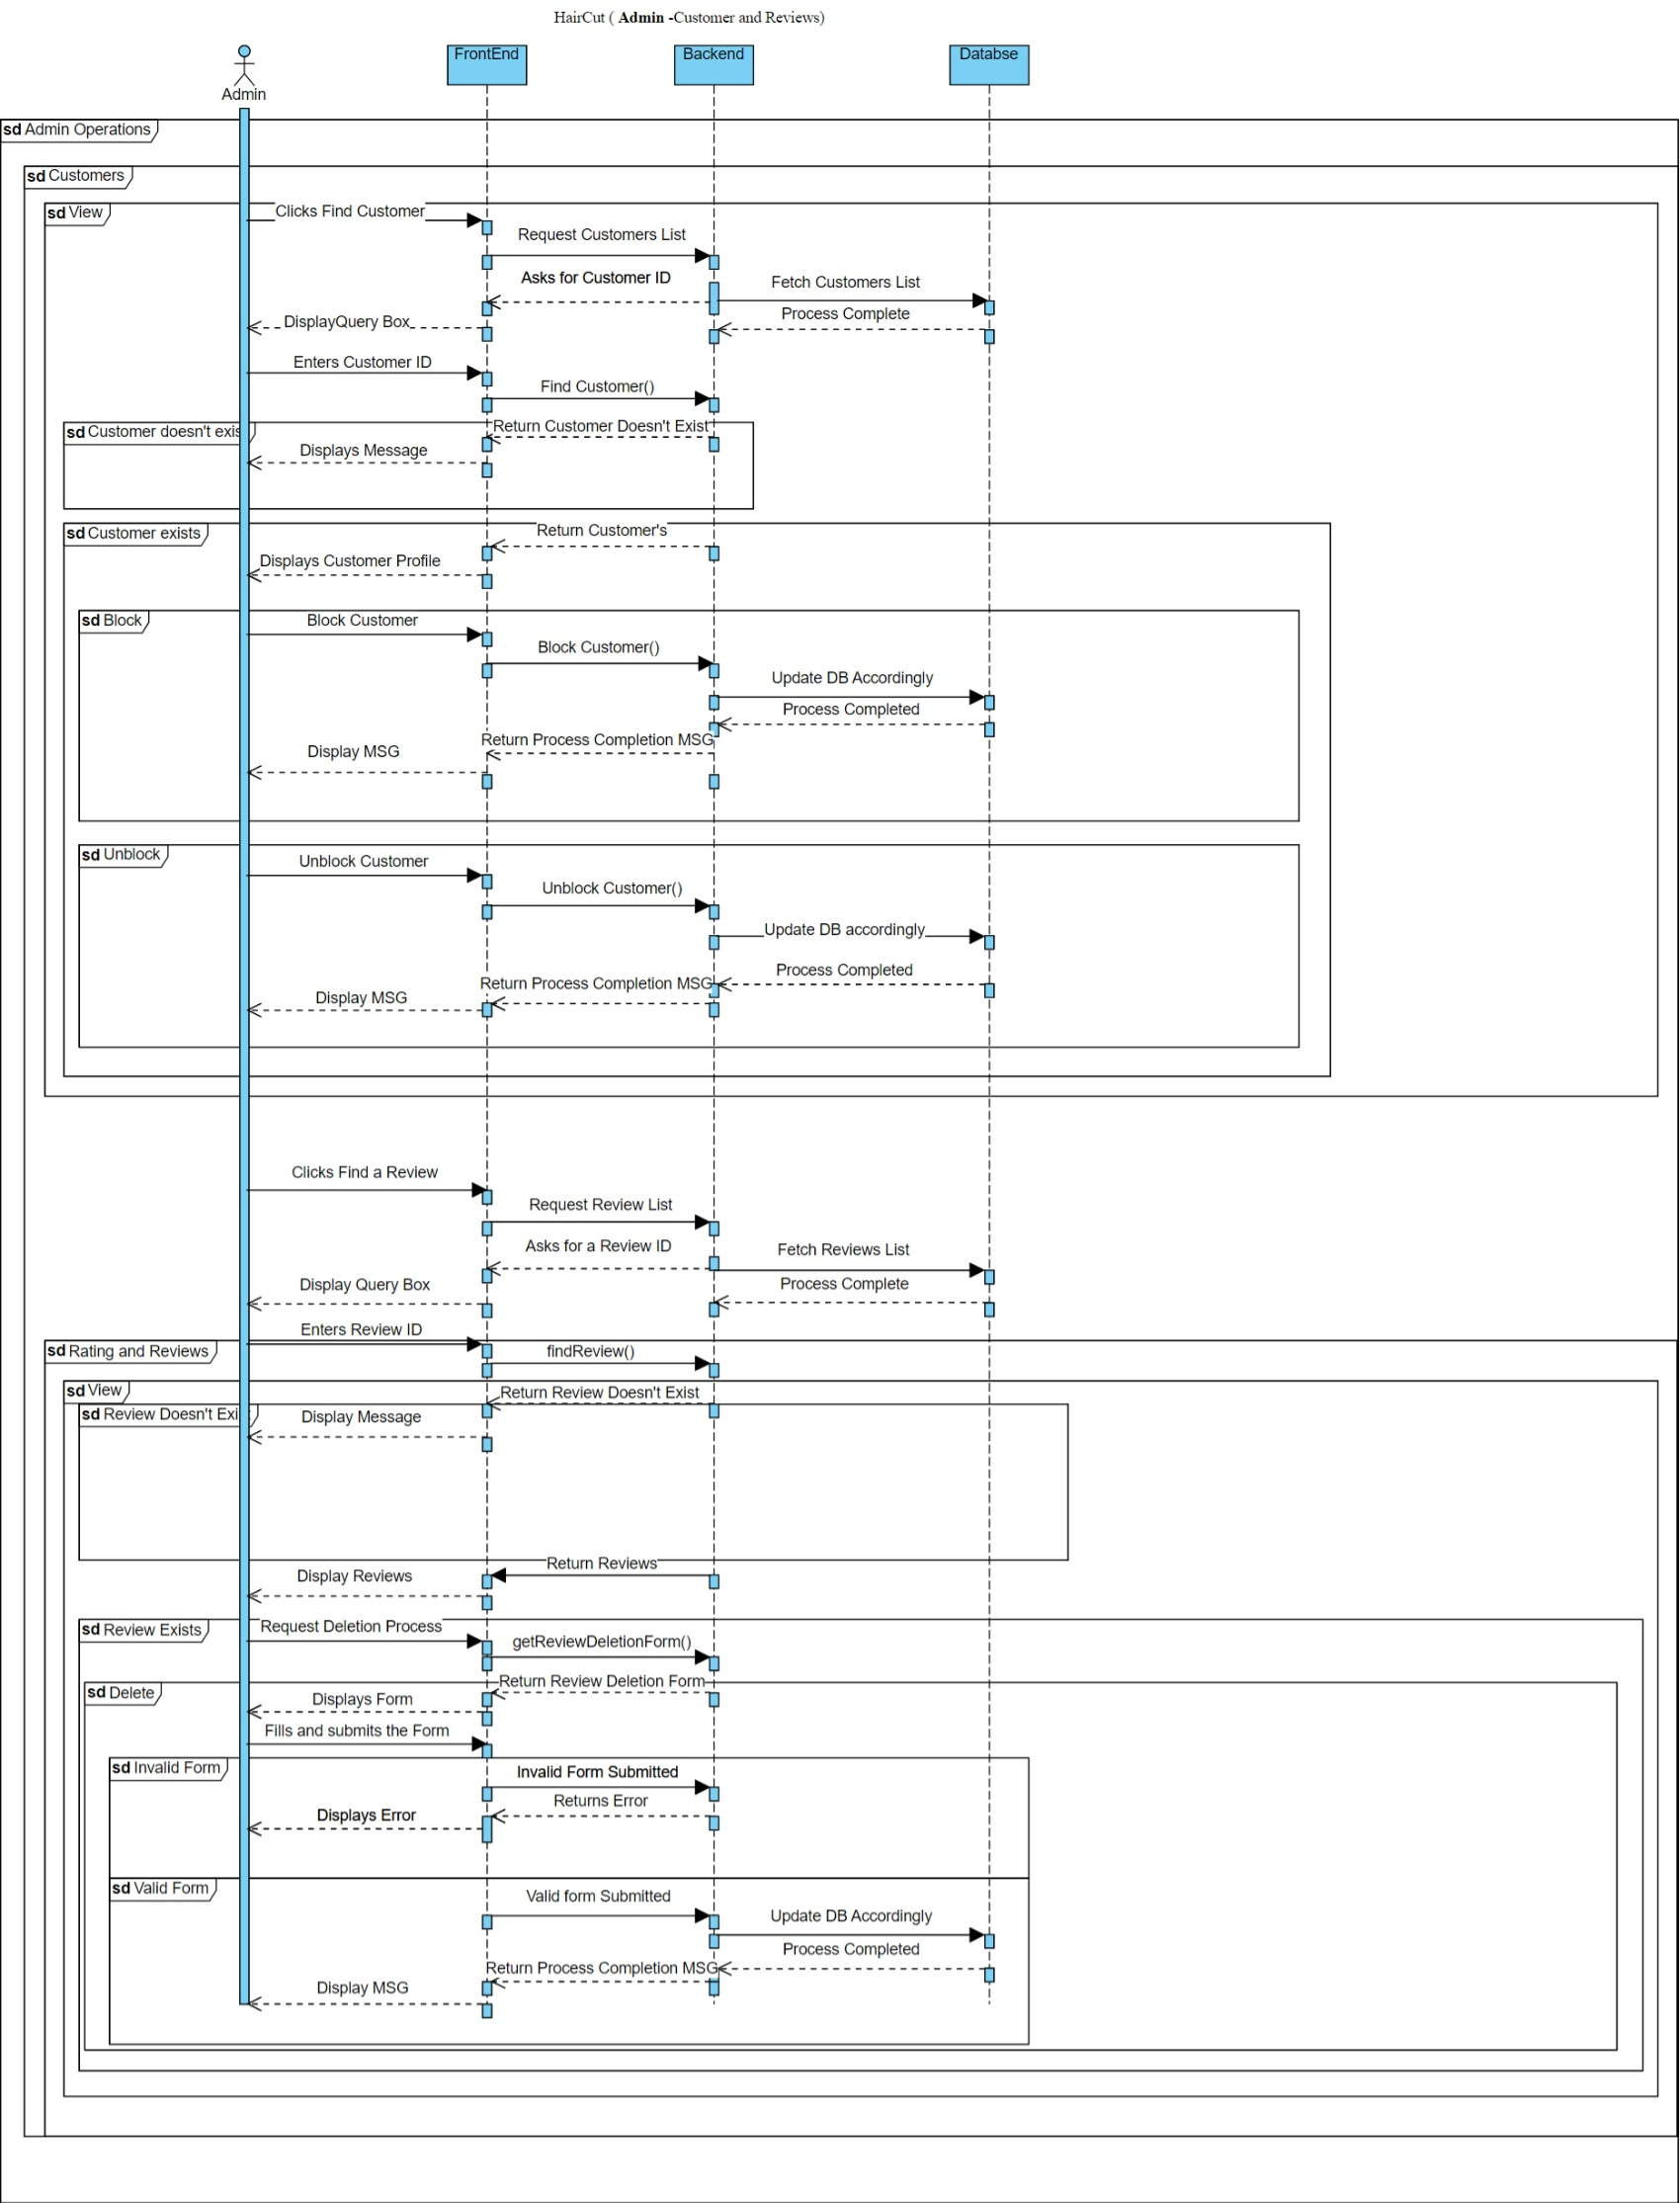
\includegraphics[width=0.75\linewidth]{images/Sequence_Diagram_5_Admin-Operations-customers-reviews.jpg}
        \caption{Sequence Diagram 5: [Admin Diagram 2] Admin operations on customers \& reviews}
    \end{figure}
      
      \subsection{User Interface Design}
      
       In this section, we are going to display the user interface and screens, starting with the log in, all the way to the payment and review. As for the customer/client registration, the customer/client chooses Register, then register as a client:
       \begin{figure}[H]
           \centering
           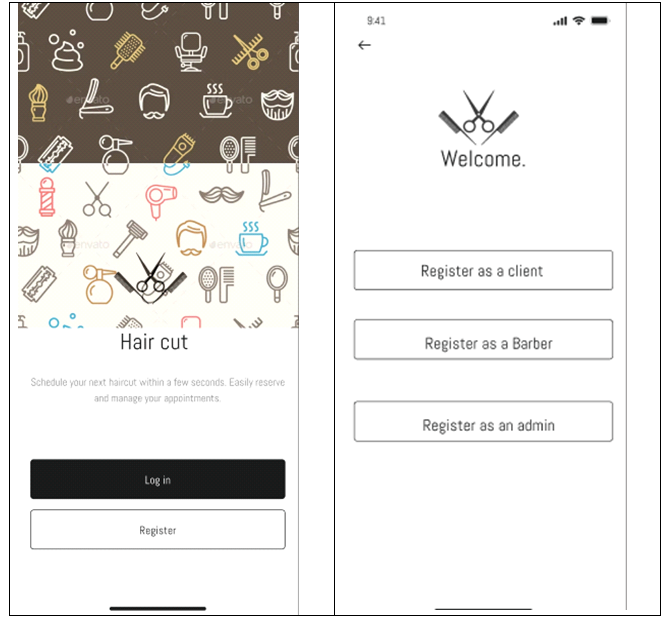
\includegraphics[width=0.75\linewidth]{images/ui1.png}
           \caption{Enter Caption}
       \end{figure}
            After he registers as client, he enters his personal information, then he uploads his picture or choose the default picture:
      \begin{figure}[H]
          \centering
          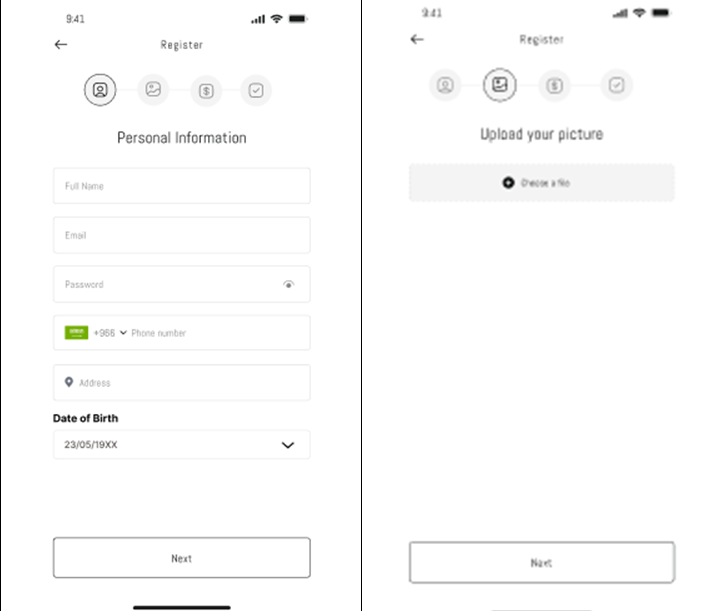
\includegraphics[width=0.75\linewidth]{images/ui2.png}
          \caption{Enter Caption}
      \end{figure}
                After he uploads his picture or choose the default picture, he enters his payment method, and finally, agree to the terms and conditions of the application:
                \begin{figure}[H]
                    \centering
                    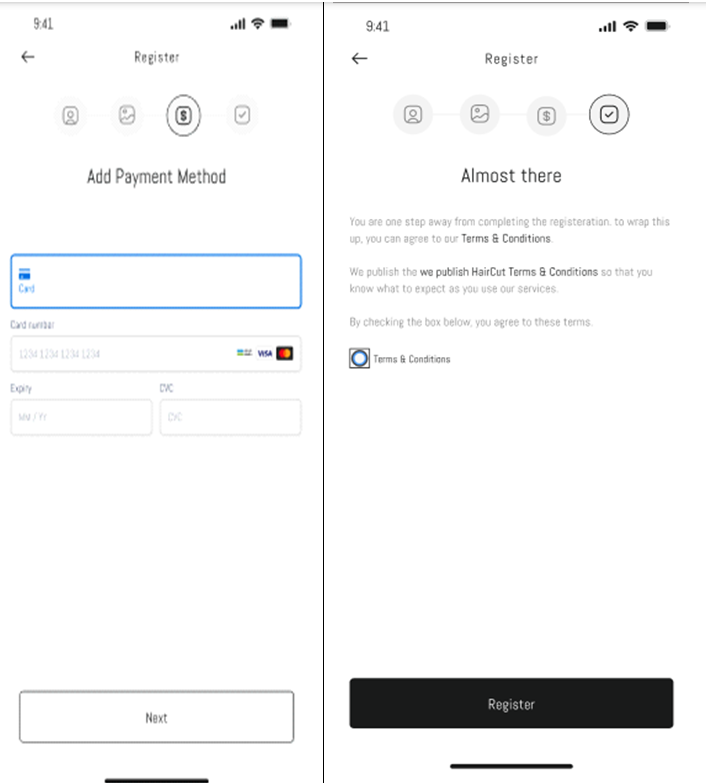
\includegraphics[width=0.75\linewidth]{images/ui3.png}
                    \caption{Enter Caption}
                \end{figure}
              As for the customer/client log in, he enters his name or phone number, and then enters his password:
              \begin{figure}[H]
                  \centering
                  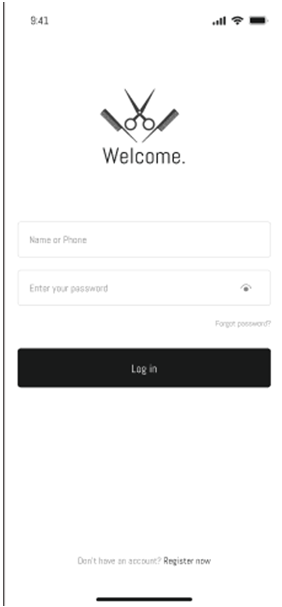
\includegraphics[width=0.65\linewidth]{images/ui4.png}
                  \caption{Enter Caption}
              \end{figure}
                     If the customer forgets his password:
                     \begin{figure}[H]
                         \centering
                         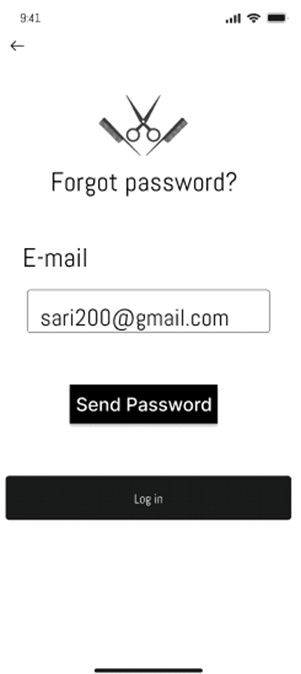
\includegraphics[width=0.60\linewidth]{images/ui5.png}
                         \caption{Enter Caption}
                     \end{figure}
      
                 As for the barber registration, the barber chooses register, then register as a barber: 
                 \begin{figure}[H]
                     \centering
                     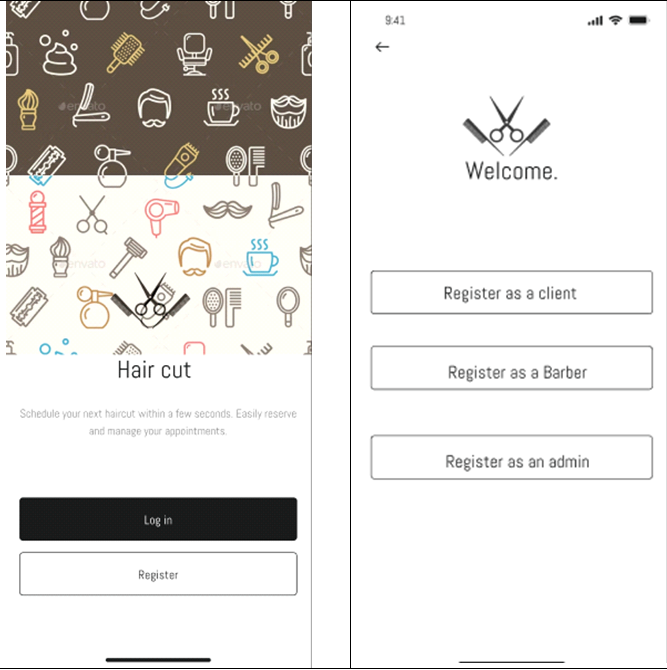
\includegraphics[width=0.65\linewidth]{images/ui6.png}
                     \caption{Enter Caption}
                 \end{figure}
      
      
               After he registers as a barber, he enters his personal information and then uploads his picture:
      \begin{figure}[H]
          \centering
          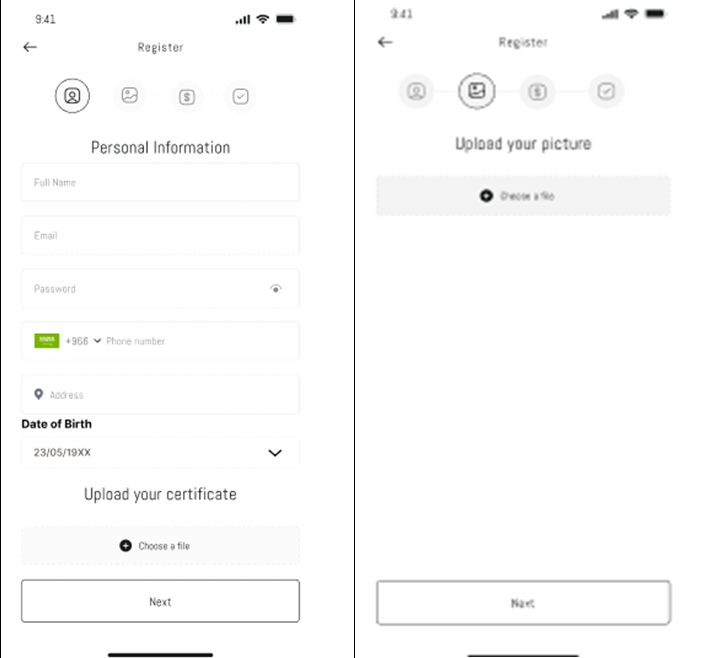
\includegraphics[width=0.75\linewidth]{images/ui7.png}
          \caption{Enter Caption}
      \end{figure}
      
               After he uploads his picture, he adds a payment method, so he receives payment, then finally, he agrees to the terms and conditions of the application:
               \begin{figure}[H]
                   \centering
                   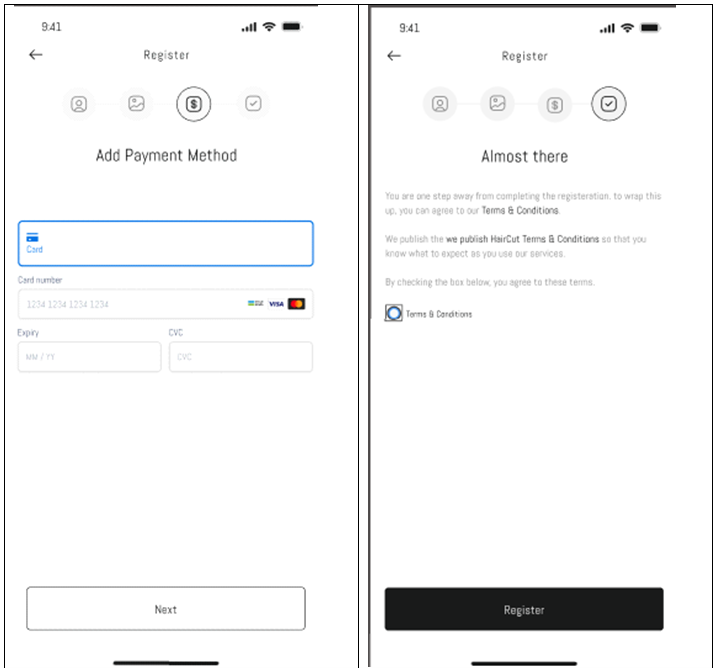
\includegraphics[width=0.75\linewidth]{images/ui8.png}
                   \caption{Enter Caption}
               \end{figure}
      
      
      
                As for the barber log in, he enters his name or phone number, and then enters his password, and if the barber forgets his password:
                \begin{figure}[H]
                    \centering
                    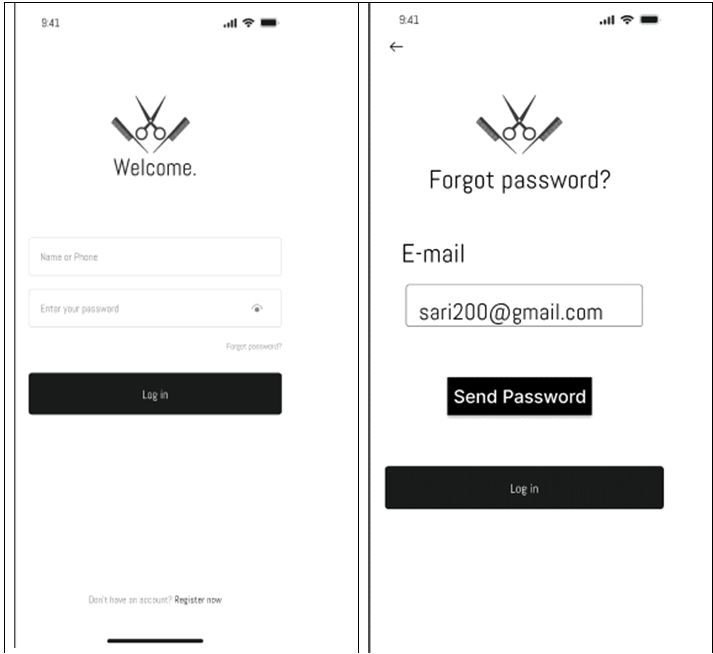
\includegraphics[width=0.75\linewidth]{images/ui9.png}
                    \caption{Enter Caption}
                \end{figure}
      
      
      
                As for the admin registration, the admin chooses register, then register as an admin:
      \begin{figure}[H]
          \centering
          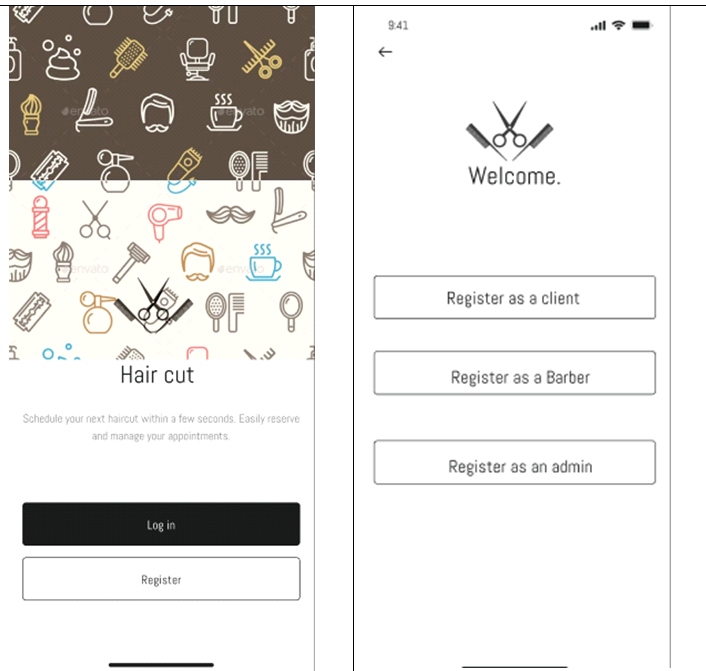
\includegraphics[width=0.75\linewidth]{images/ui10.png}
          \caption{Enter Caption}
      \end{figure}
      
      
                 After he registers as an admin, he enters his personal information, then he uploads his picture:
      \begin{figure}[H]
          \centering  
          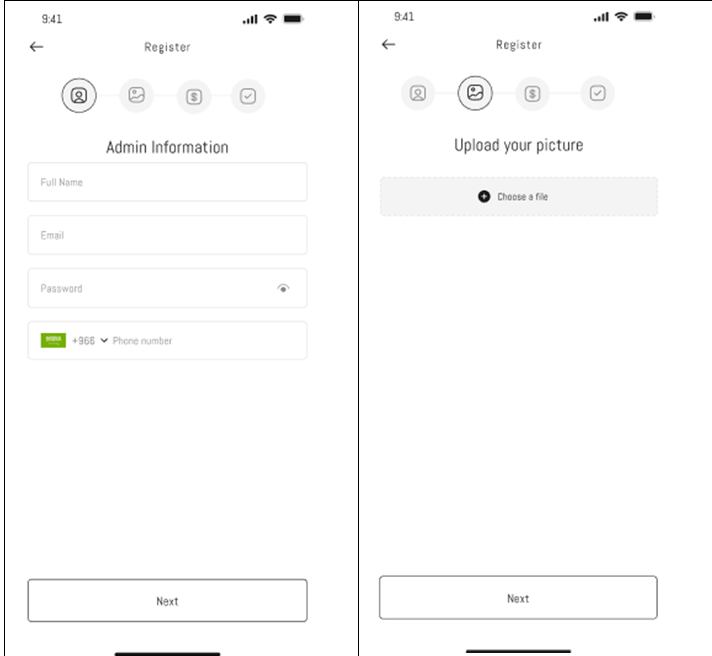
\includegraphics[width=0.75\linewidth]{images/ui11.png}
          \caption{Enter Caption}
      \end{figure}
                And finally, he agrees to the terms and conditions of the application:
                \begin{figure}[H]
                    \centering
                    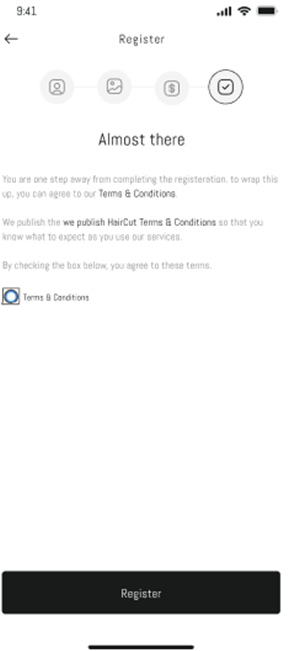
\includegraphics[width=0.65\linewidth]{images/ui12.png}
                    \caption{Enter Caption}
                \end{figure}
      
                   As for the admin log in, he enters his name or phone number, and then enters his password, and if the admin forgets his password:
                   \begin{figure}[H]
                       \centering
                       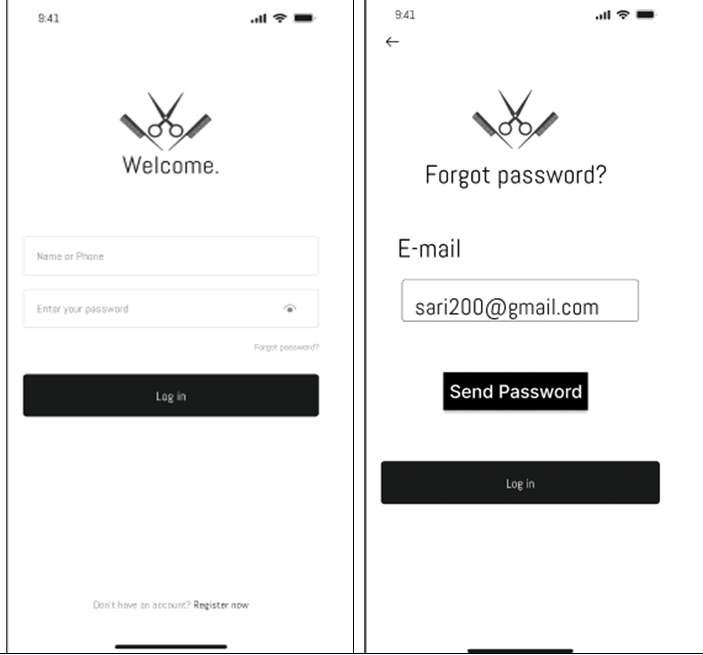
\includegraphics[width=0.75\linewidth]{images/ui13.png}
                       \caption{Enter Caption}
                   \end{figure}
      
      
      
               As for the customer/client interface, information is shown about nearby barbershops, and popular barbershops as well:
              \begin{figure}[H]
                  \centering
                  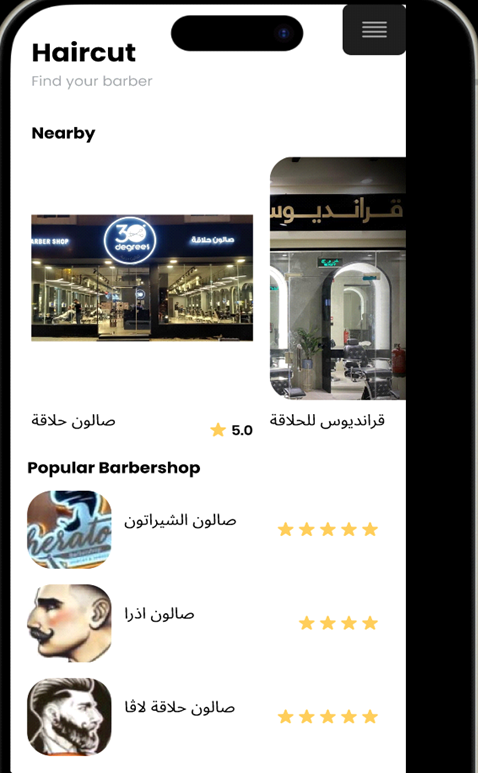
\includegraphics[width=0.75\linewidth]{images/ui14.png}
                  \caption{Enter Caption}
              \end{figure}
      On the top right corner, the customer/client can view profile or about us section, we are going to show the about us section first:
      \begin{figure}[H]
          \centering
          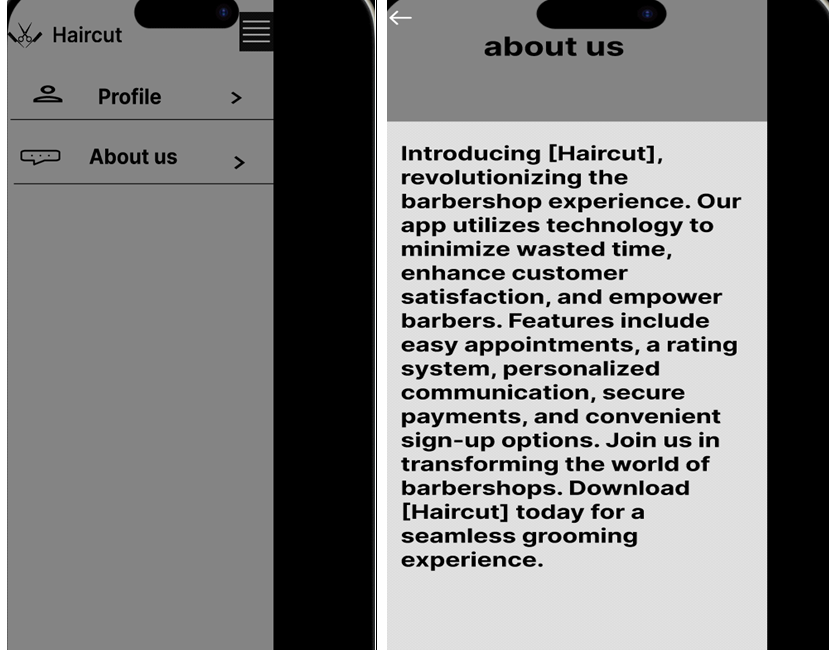
\includegraphics[width=0.75\linewidth]{images/ui15.png}
          \caption{Enter Caption}
      \end{figure}
      
                 As for the profile, the customer/client can view their profile and edit their profile:
      \begin{figure}[H]
          \centering
          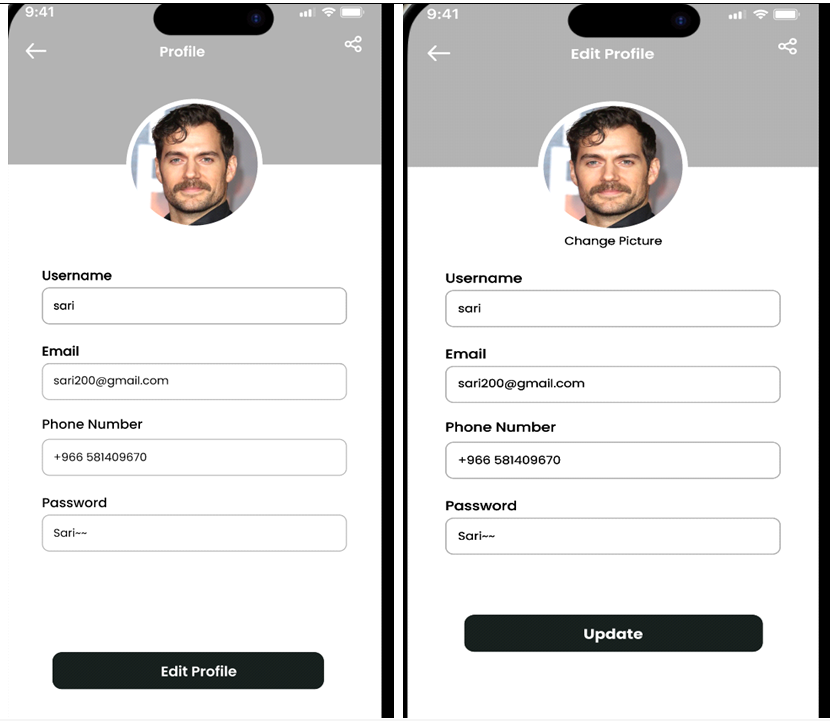
\includegraphics[width=0.75\linewidth]{images/ui16.png}
          \caption{Enter Caption}
      \end{figure}
                 
                 After the customer/client chooses the barbershop, they can view the services, set appointments, contact the barber, make payment, and finally leave a review:
                 \begin{figure}[H]
                     \centering
                     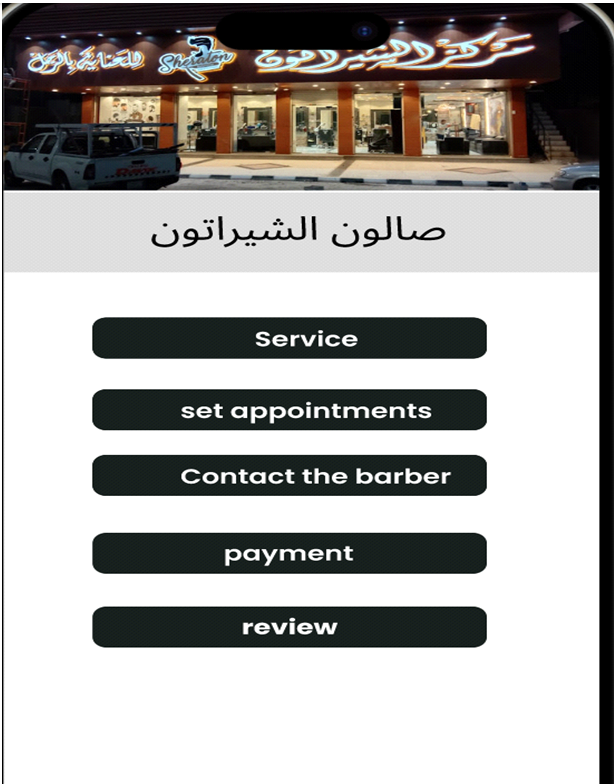
\includegraphics[width=0.75\linewidth]{images/ui17.png}
                     \caption{Enter Caption}
                 \end{figure}
      
            The customer/client can view the services provided by the barbershop:
      \begin{figure}[H]
          \centering
          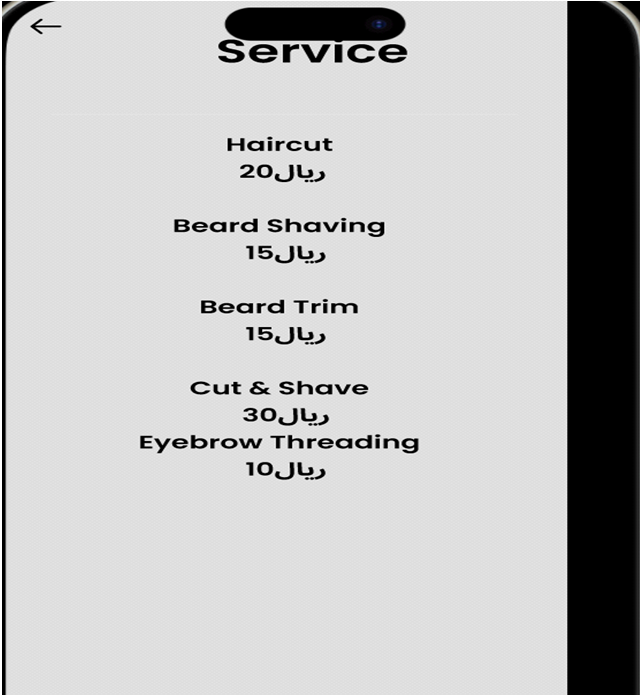
\includegraphics[width=0.75\linewidth]{images/ui18.png}
          \caption{Enter Caption}
      \end{figure}
      
               After viewing the service, the customer/client can set appointments:
               \begin{figure}[H]
                   \centering
                   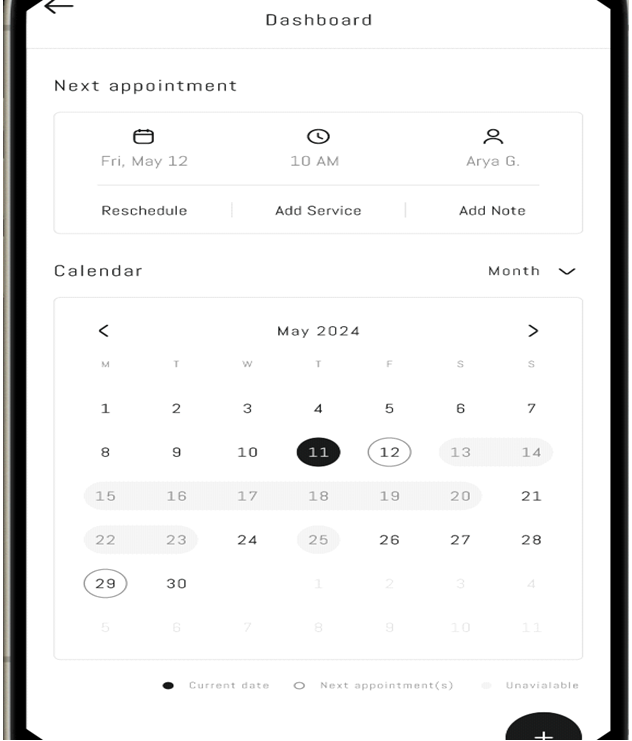
\includegraphics[width=0.75\linewidth]{images/ui19.png}
                   \caption{Enter Caption}
               \end{figure}
      
                The customer/client can also contact the barber/barbershop:
                \begin{figure}[H]
                    \centering
                    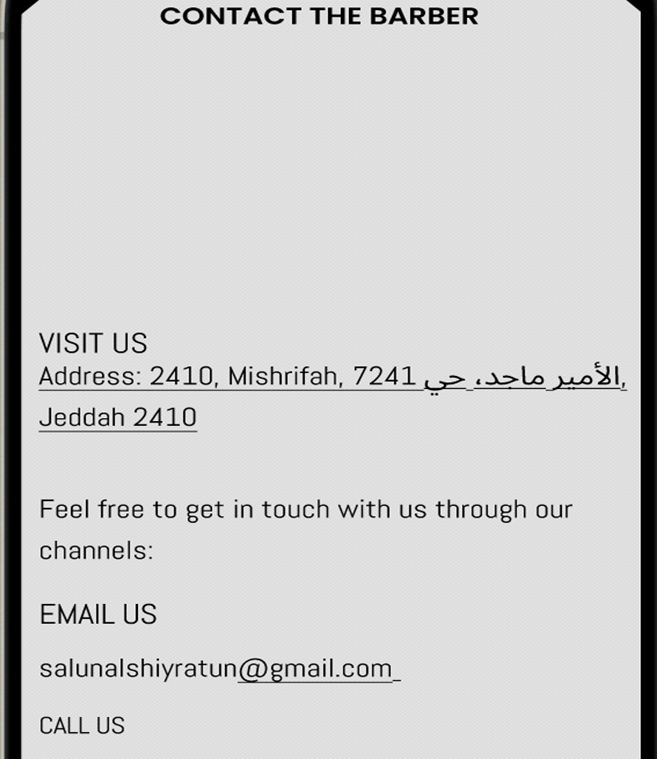
\includegraphics[width=0.75\linewidth]{images/ui20.png}
                    \caption{Enter Caption}
                \end{figure}
      
                After the customer/client contacts the barber/barbershop and sets the appointment, the customer can choose the service he wants and then make the payment/place the order:
      \begin{figure}[H]
          \centering
          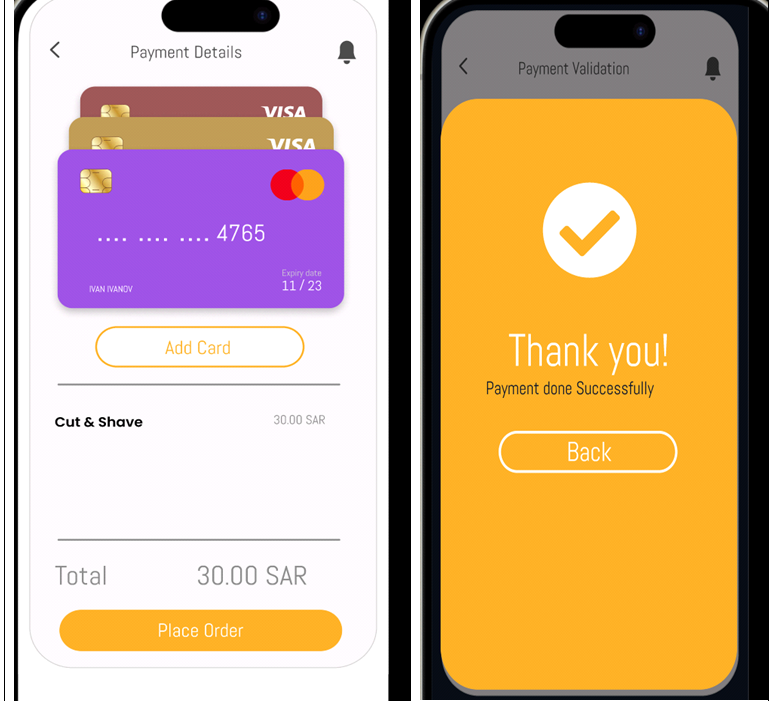
\includegraphics[width=0.75\linewidth]{images/ui21.png}
          \caption{Enter Caption}
      \end{figure}
           After receiving the service, the customer/client can leave a review on the service provided:
          \begin{figure}[H]
              \centering
              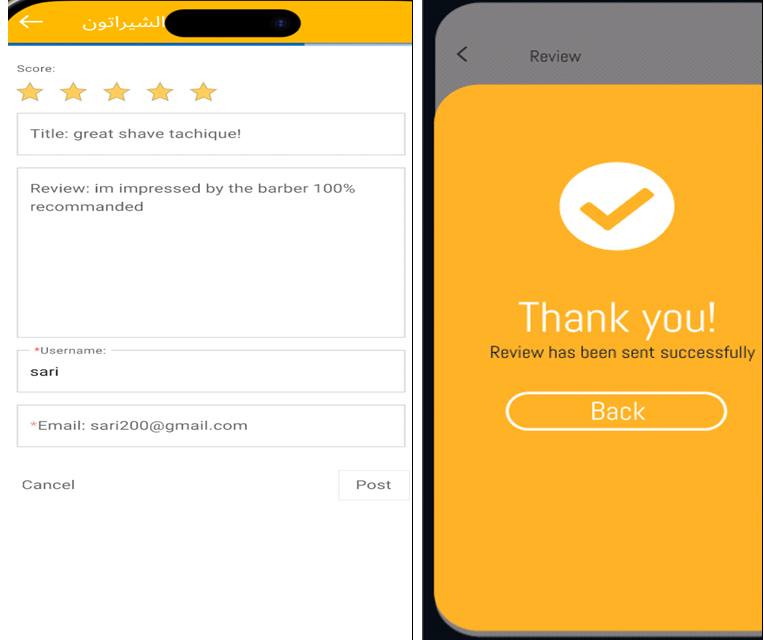
\includegraphics[width=0.75\linewidth]{images/ui22.png}
              \caption{Enter Caption}
          \end{figure}
                \begin{figure}[H]
                    \centering
                    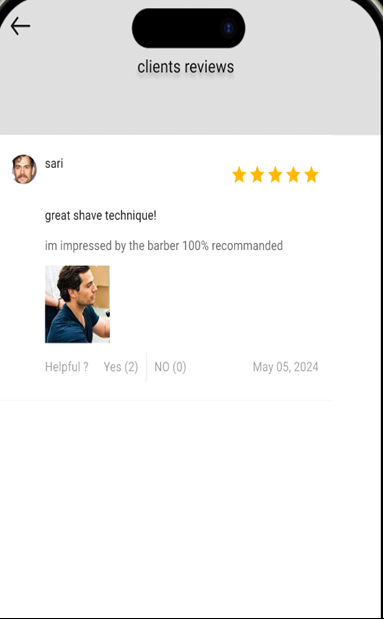
\includegraphics[width=0.75\linewidth]{images/ui23.png}
                    \caption{Enter Caption}
                \end{figure}
                As for the barber interface, information is shown barbershop, the barber can view his profile, edit services, see appointments, edit contact information, payment, checking reviews, and sign out of the application:
                
      \begin{figure}[H]
          \centering
          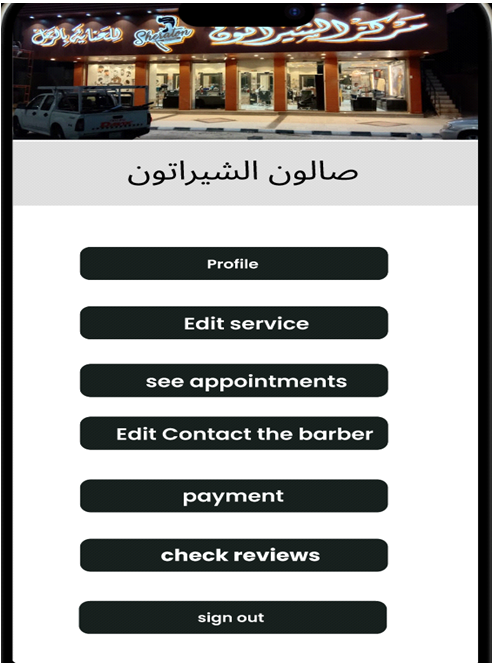
\includegraphics[width=0.75\linewidth]{images/ui24.png}
          \caption{Enter Caption}
      \end{figure}
            The barber can view and edit his profile:
      \begin{figure}[H]
          \centering
          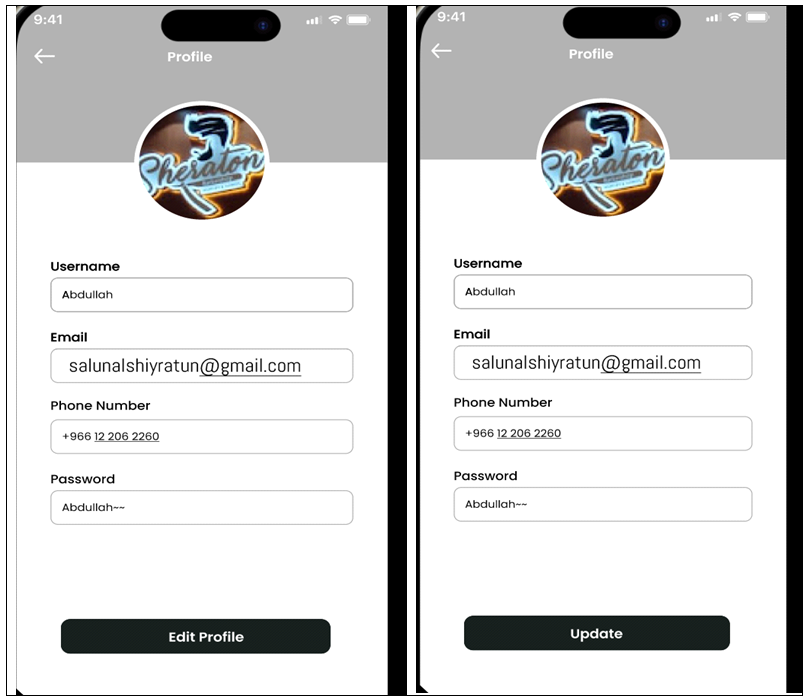
\includegraphics[width=0.75\linewidth]{images/ui25.png}
          \caption{Enter Caption}
      \end{figure}
      
      
              The barber can edit his service and see appointments made:
      \begin{figure}[H]
          \centering
          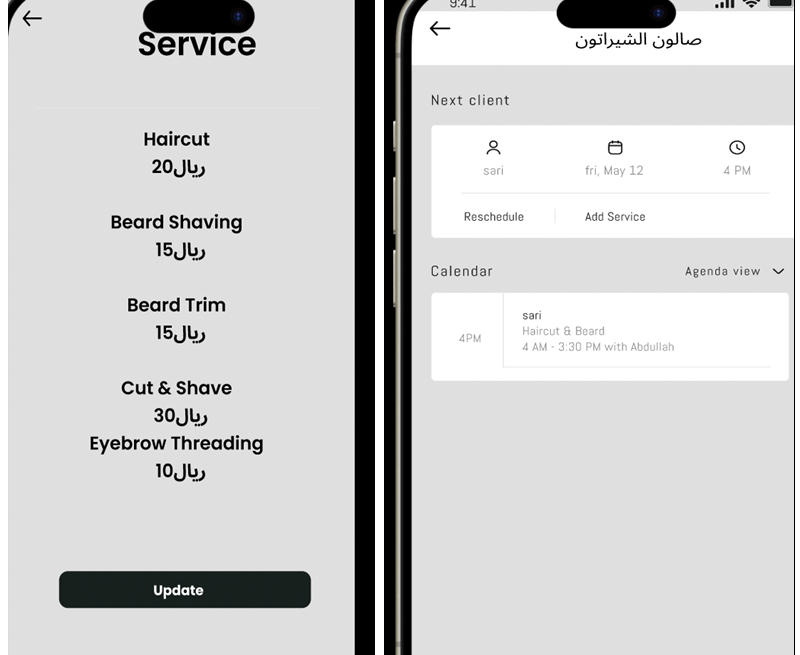
\includegraphics[width=0.75\linewidth]{images/ui26.png}
          \caption{Enter Caption}
      \end{figure}
                
                The barber can edit his contact information and view payments made by customers/clients:
      \begin{figure}[H]
          \centering
          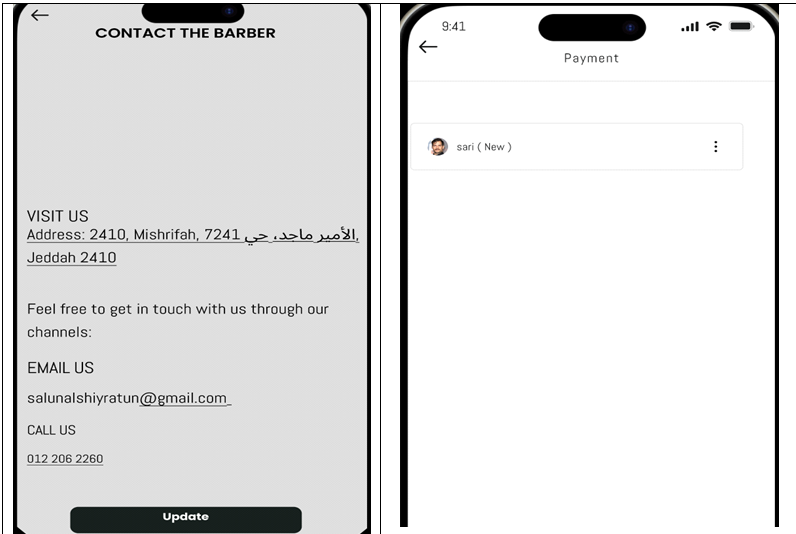
\includegraphics[width=0.75\linewidth]{images/ui27.png}
          \caption{Enter Caption}
      \end{figure}
      \begin{figure}[H]
          \centering
          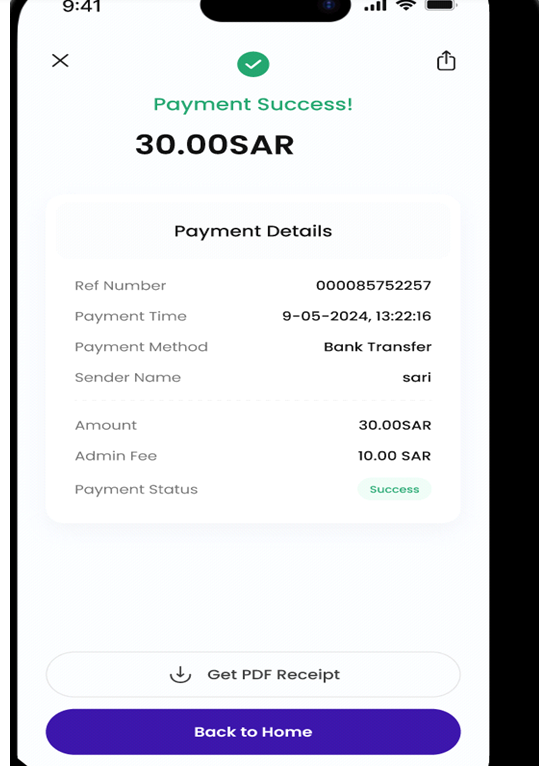
\includegraphics[width=0.75\linewidth]{images/ui28.png}
          \caption{Enter Caption}
      \end{figure}
           The barber can check reviews made by clients/customers and sign out of the application, once the barber signs out, he will be returned to the log in page:
      \begin{figure}[H]
          \centering
          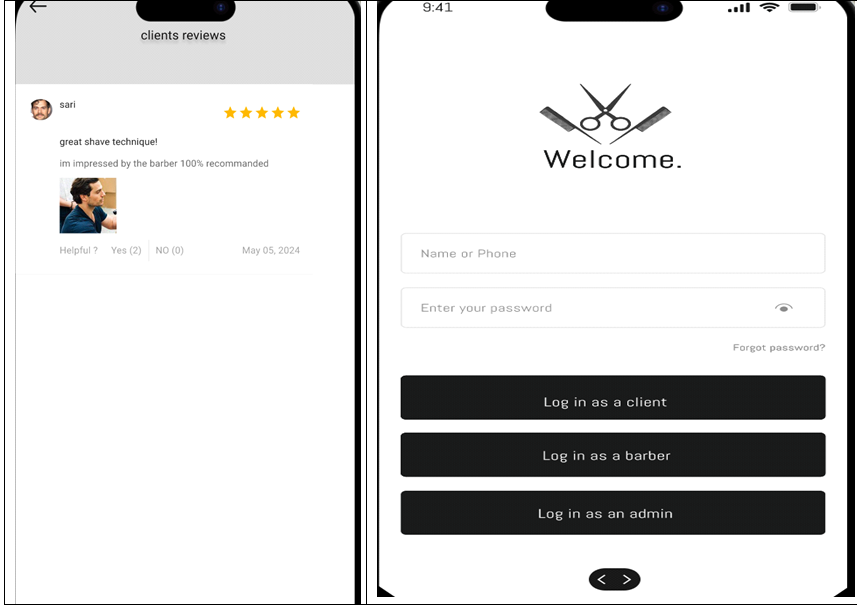
\includegraphics[width=0.75\linewidth]{images/ui29.png}
          \caption{Enter Caption}
      \end{figure}
                   As for the admin interface, the admin can view the barber profile and view the client/customer rating/review:
      \begin{figure}[H]
          \centering
          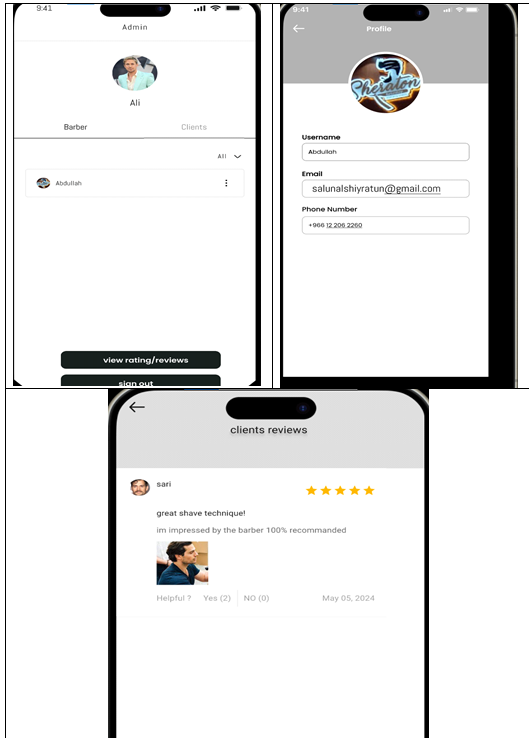
\includegraphics[width=1\linewidth]{images/ui30.png}
          \caption{Enter Caption}
      \end{figure}
      
       The admin can view the customer profile and view the barber rating/review and the admin can sign out of the application, once he signs out of the application, he will be returned to the log in page:
      
      \begin{figure}[H]
          \centering
          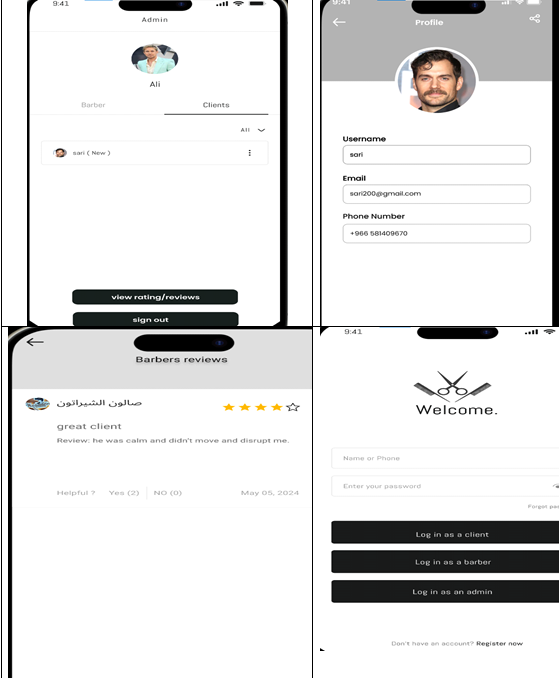
\includegraphics[width=1\linewidth]{images/ui31.png}
          \caption{Enter Caption}
      \end{figure}
      
      \section{Conclusion}
      In conclusion, we have discussed in this chapter the detailed design of the application, starting with the static aspect design using a class diagram to display the functional and non-functional requirements,
      the architectural aspect design, the dynamic aspect design, and finally the user interface design, this concludes our final chapter.
      \section{References}
      \subsection{Chapter 2: Existing systems:} 
      \begin{itemize}
        \item Acuity Scheduling: \href{https://acuityscheduling.com/\#gref}{https://acuityscheduling.com/\#gref}
        \item DaySmart Salon: \href{https://www.daysmart.com/salon/}{https://www.daysmart.com/salon/}
        \item \href{ https://www.mindbodyonline.com/en-gb/business/lp/mindbody?landing=y&utm_source=google&utm_medium=ppc&utm_campaign=20430748488&ad_group=160722387588&utm_term=kwd-329860702&utm_device=c&referralSource=paid+search&matchtype=e&cid=685008699808&networkType=search&adgroupid=160722387588&creative=685008699808&network=g&adGroup=160722387588&_bk=mindbody&_bm=e&gad_source=1&gclid=Cj0KCQiArrCvBhCNARIsAOkAGcXkhoxZN2kd43kY-JN37kZmb38xqd5jLQhS4T8uUtLw5eR_OVGaqy4aAlL3EALw_wcB}{MindBodyOnline}
        \item Vagaro: \href{https://www.vagaro.com/pro/about-us}{https://www.vagaro.com/pro/about-us}
        \item WellnessLiving: \href{https://www.wellnessliving.com/}{https://www.wellnessliving.com/}
        \item Zenoti: \href{https://www.zenoti.com/}{https://www.zenoti.com/}
        \item TheCut App: \href{https://www.thecut.co/}{https://www.thecut.co/}
        \item Setmore: \href{https://www.setmore.com/}{https://www.setmore.com/}
        \item StyleSeat: \href{https://www.styleseat.com/m/}{https://www.styleseat.com/m/}
        \item Square Appointments: \href{https://squareup.com/us/en/appointments}{https://squareup.com/us/en/appointments}
        \item Schedulicity: \href{https://www.schedulicity.com/}{https://www.schedulicity.com/}  
        \item Home service: \url{https://www.researchgate.net/publication/358571278_In-Home_Service_Consumption_A_Systematic_Review_Integrative_Framework_and_Future_Research_Agenda}
        \item User-Friendly interface: \href{https://doi.org/10.1155/2017/6787504}{https://doi.org/10.1155/2017/6787504}
        \item Convenient appointment booking: \url{https://www.primescholars.com/articles/literature-review-on-appointment-scheduling-in-hospitals-management.pdf}
        \item Automated Reminders/alerts: \href{https://www.ncbi.nlm.nih.gov/pmc/articles/PMC4912908/}{https://www.ncbi.nlm.nih.gov/pmc/articles/PMC4912908/}
        \item Payment system: \url{https://www.researchgate.net/publication/329838236_A_Review_of_E-Payment_System_in_E-Commerce}
        \item Rating/Review System: \url{https://www.researchgate.net/publication/317631936_An_Examination_of_the_Current_Rating_System_used_in_Mobile_App_Stores}
    \end{itemize}
    \subsection{Chapter 3: General Analysis}
    \begin{itemize}
        \item Requirements Gathering google form: \href{https://docs.google.com/forms/d/e/1FAIpQLSes28stJGbO_i-1EmL-VT60-TKeAUTfT0DXHwRMSb1ncaQepA/viewform?usp=sf_link}{https://docs.google.com/forms/d/e/1FAIpQLSes28stJGbO\_i-1EmL-VT60-TKeAUTfT0DXHwRMSb1ncaQepA/viewform?usp=sf\_link}
        \item Use case diagram: \href{https://lucid.app/lucidchart/invitations/accept/inv_47530d0c-9e96-43cc-8c8e-ea354d96ebdf}{https://lucid.app/lucidchart/invitations/accept/inv\_47530d0c-9e96-43cc-8c8e-ea354d96ebdf}
        \item Dynamic Diagram (Activity Diagram) \url{https://lucid.app/lucidchart/invitations/accept/inv_e6a319dc-4328-489a-9ac8-e24d1eb38706}
    \end{itemize}
    \subsection{Chapter 4: Detailed Desgin}
    \begin{itemize}
       \item User interface design: \href{https://www.figma.com/proto/vcdFPDnXduhTrPKnwB27uj/Haircut?node-id=2-11&t=U3ZWMewK0ODQ4fIH-1&scaling=scale-down&page-id=0%3A1&starting-point-node-id=2%3A11&show-proto-sidebar=1}{User interface design}
    \end{itemize}
\end{document}
